\chapter{Welded Connections}
\section{Basic Types of Welded Joint}
\begin{figure}[H]
\centering
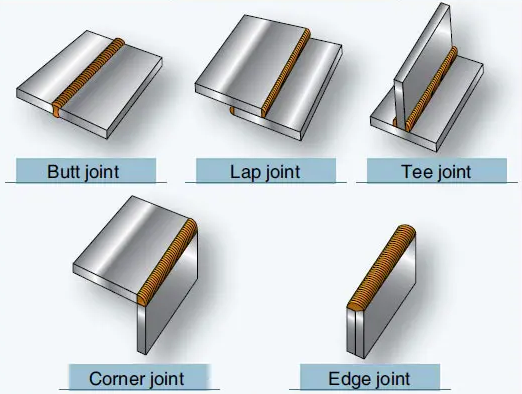
\includegraphics[scale=.7]{PIC/CH07/WT}
\caption{Basic types of welded joints (\href{https://www.flight-mechanic.com/welded-joints-using-oxy-acetylene-torch/}{\url{https://www.flight-mechanic.com/welded-joints-using-oxy-acetylene-torch/}})}
\end{figure}
Lapped joints are the most common. Here are some examples.
\begin{figure}[H]
\footnotesize\centering
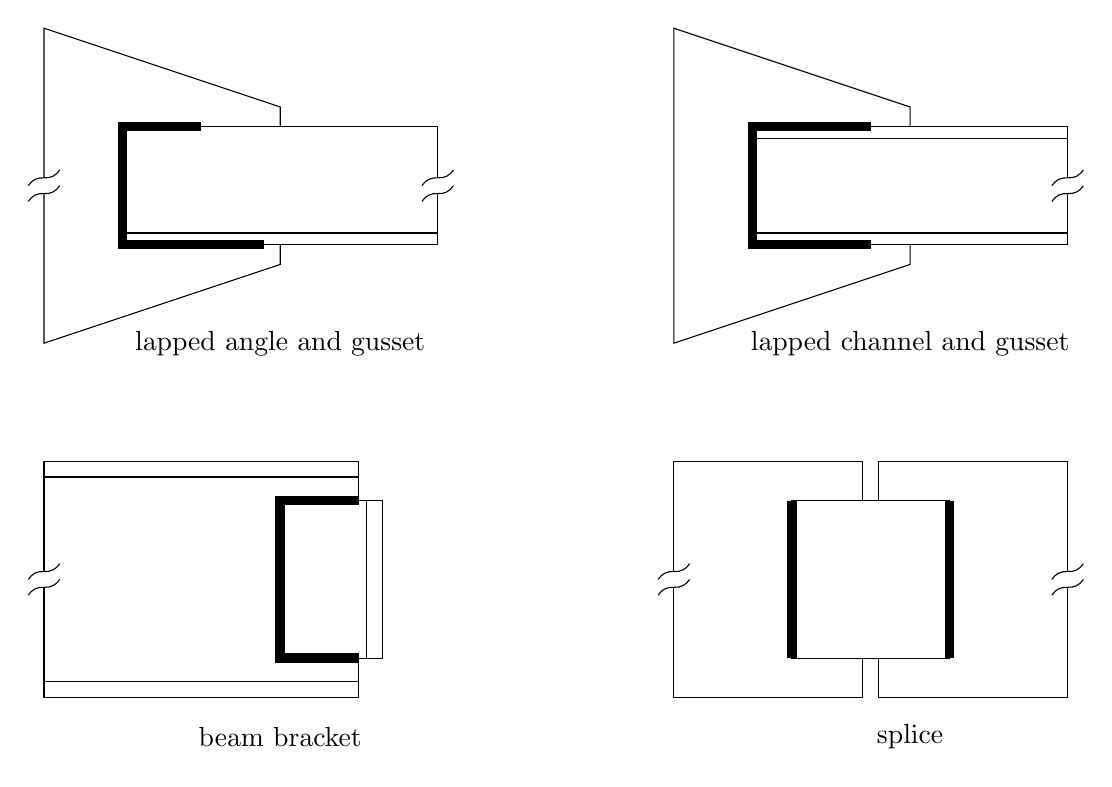
\begin{tikzpicture}[scale=1,ext/.pic={
\path[fill=white](-0.2,0)to[bend left](0,0.1)to[bend right](0.2,0.2)to(0.2,0)to[bend left](0,-0.1)to[bend right](-0.2,-0.2)--cycle;
\draw(-0.2,0)to[bend left](0,0.1)to[bend right](0.2,0.2) (0.2,0)to[bend left](0,-0.1)to[bend right](-0.2,-0.2);
}]
\draw(2,-1)--(2,1)--(-1,2)--(-1,-2)--cycle;
\draw[fill=white](0,-.75)rectangle(4,.75);
\draw(0,-.6)--(4,-.6);
\draw(4,0)pic{ext}(-1,0)pic{ext};
\draw[line width=1.2mm](1,.75)-|(0,-.75)--++(1.8,0);
\node at(2,-2){lapped angle and gusset};
\begin{scope}[xshift=8cm]
\draw(2,-1)--(2,1)--(-1,2)--(-1,-2)--cycle;
\draw[fill=white](0,-.75)rectangle(4,.75);
\draw(0,-.6)--(4,-.6)(0,.6)--(4,.6);
\draw(4,0)pic{ext};(-1,0)pic{ext};
\draw[line width=1.2mm](1.5,.75)-|(0,-.75)--++(1.5,0);
\node at(2,-2){lapped channel and gusset};
\end{scope}
\begin{scope}[yshift=-5cm]
\draw(3,-1.5)rectangle(-1,1.5);
\draw(3,-1.3)--++(-4,0)(3,1.3)--++(-4,0);
\draw[fill=white](2,-1)rectangle(3.3,1);
\draw(3.1,1)--++(0,-2);
\draw(-1,0)pic{ext};
\draw[line width=1.2mm](3,-1)-|(2,1)--++(1,0);
\node at(2,-2){beam bracket};
\begin{scope}[xshift=8cm]
\draw(1.4,-1.5)rectangle(-1,1.5);
\draw(1.6,-1.5)rectangle(4,1.5);
\draw[fill=white](.5,-1)rectangle(2.5,1);
\draw(-1,0)pic{ext}(4,0)pic{ext};
\draw[line width=1.2mm](.5,-1)--++(0,2)(2.5,-1)--++(0,2);
\node at(2,-2){splice};
\end{scope}
\end{scope}
\end{tikzpicture}
\caption{Examples of lapped joints}
\end{figure}
\section{Weld Categories and Types}
\NZSSTEEL{} permits the use of two weld categories.
\begin{itemize}
\item GP --- General Purpose (for design $\phi=0.6$)\\For general welds where demand is less than the weld capacity.
\item SP --- Structural Purpose (for design $\phi=0.8$ but $\phi=0.9$ for butt welds)\\For welds:
\begin{itemize}
\item where demand is greater than GP weld capacity;
\item subject to high cycle fatigue loading; or
\item in main framing subjecting to earthquake loading.
\end{itemize}
\end{itemize}
GP welds allow larger imperfections than SP welds do.

\NZSSTEEL{} deals with six types of welds as shown below.
\begin{itemize}
\item Complete penetration butt/groove weld
\begin{figure}[H]
\centering
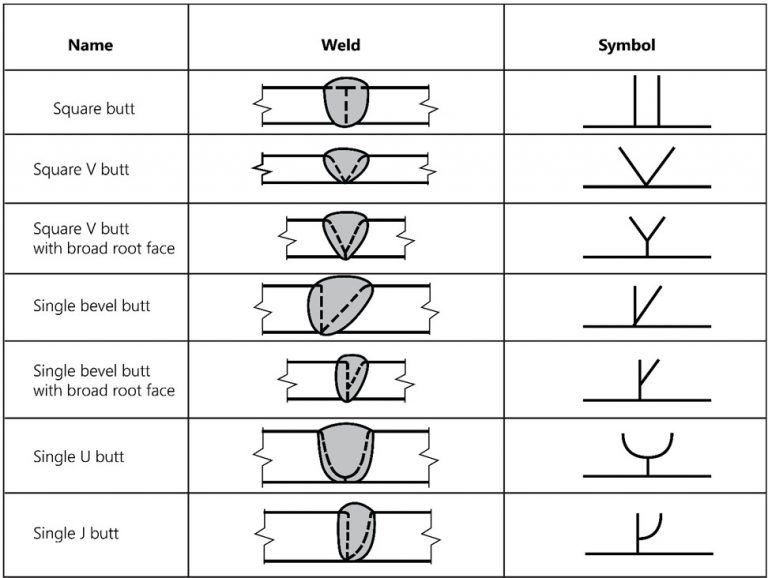
\includegraphics[scale=.6]{PIC/CH07/WE}
\end{figure}
\item Incomplete penetration butt/groove weld (not at a corner or T-joint)
\begin{figure}[H]
\centering
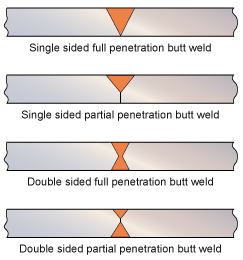
\includegraphics[scale=.6]{PIC/CH07/PW}
\end{figure}
\item Fillet weld
\begin{figure}[H]
\centering
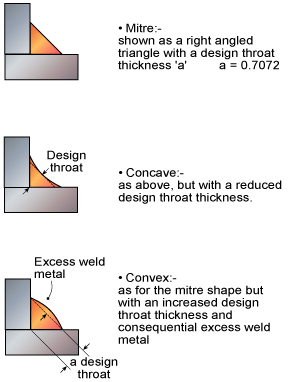
\includegraphics[scale=.6]{PIC/CH07/FW3}
\end{figure}
\item Compound weld
\begin{figure}[H]
\centering
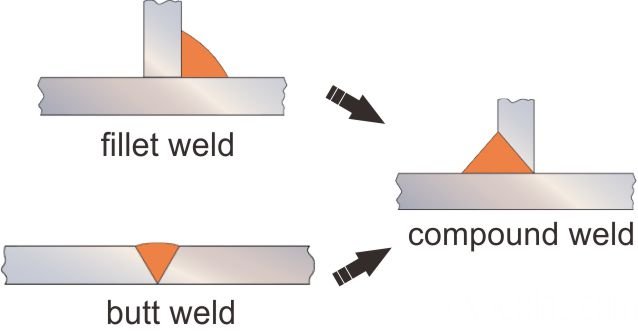
\includegraphics[scale=1]{PIC/CH07/CW}
\end{figure}
\item Plug weld
\begin{figure}[H]
\centering
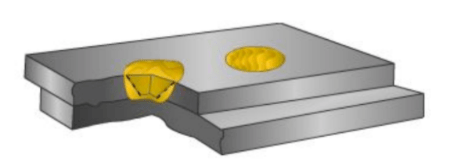
\includegraphics[scale=.6]{PIC/CH07/PLUG}
\end{figure}
\item Slot weld
\begin{figure}[H]
\centering
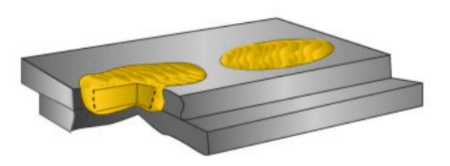
\includegraphics[scale=.6]{PIC/CH07/SLOT}
\end{figure}
\end{itemize}
\section{Weld Process}
Welding is \textbf{a materials joining process which produces coalescence of materials by heating the to suitable temperatures}.

Heat is used to melt the base material and a filler material in order that flow of material will occur and that fusion will take place.

Several welding processes are available. The most common are
\begin{itemize}
\item Shield Metal Arc Welding (SMAW)
\begin{figure}[H]\centering
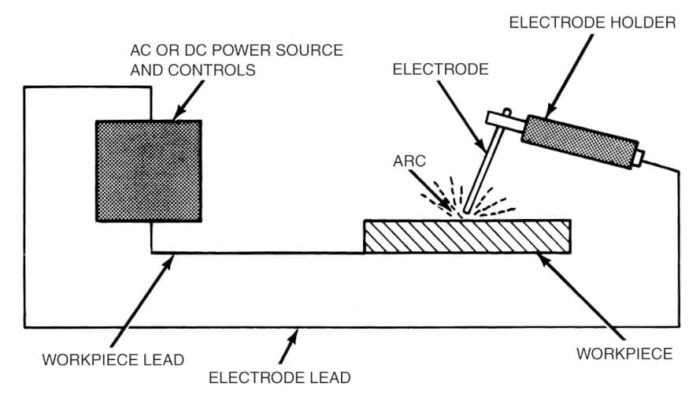
\includegraphics[width=10cm]{PIC/CH07/SMAW1}
\caption{Shield metal arc welding (\href{https://www.fabtechexpo.com/blog/2018/01/04/shielded-metal-arc-welding-basics}{\url{https://www.fabtechexpo.com/blog/2018/01/04/shielded-metal-arc-welding-basics}})}
\end{figure}
\begin{figure}[H]\centering
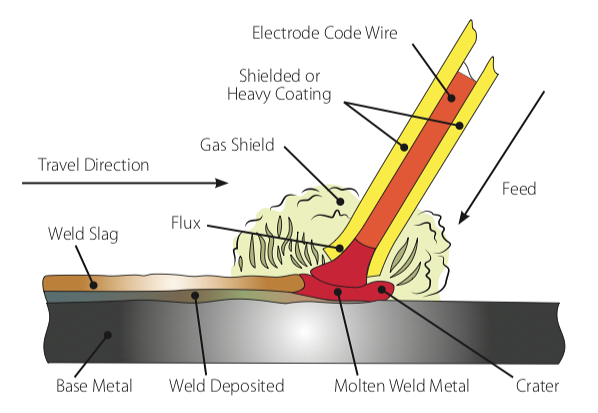
\includegraphics[width=10cm]{PIC/CH07/SMAW}
\caption{Shield metal arc welding (\href{https://www.jasic.co.uk/guide-to-mma-welding}{\url{https://www.jasic.co.uk/guide-to-mma-welding}})}
\end{figure}
This includes
\begin{itemize}
\item Manual Metal Arc Welding (MMAW)\\Welding with a stick electrode with flux coating. The shielding may perform the following functions.
\begin{itemize}
\item Produce a gaseous shield to exclude air and stabilize the arc.
\item Introduce other materials, e.g., deoxidizers to refine grain structure of weld metal.
\item Produce a slag blanket to protect it from air and retard cooling.
\end{itemize}
It is slow (expensive) but versatile.
\item Gas Metal Arc Welding (GMAW)\\Welding with a steel wire fed through a gun with gas (e.g., \ce{CO2}, \ce{Ar}, \ce{O2}) shielding.

It is faster but wind dependent --- not for field welding.
\item Flux Cored Arc Welding (FCAW)\\Welding with a hollow steel wire filled with flux fed through a gun --- sometimes inert shielding as is used too.

It is fast but needs good access.
\end{itemize}
\item Submerged Arc Welding (SAW)
\begin{figure}[H]\centering
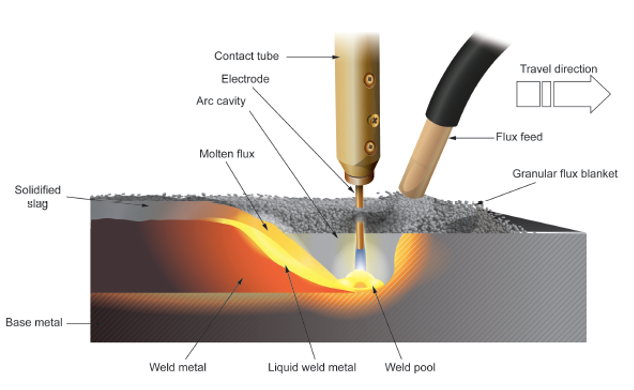
\includegraphics[scale=.9]{PIC/CH07/SAW}
\caption{Submerged arc welding (\href{https://www.cwbgroup.org/sites/default/files/imgs/saw-fig1.png}{\url{https://www.cwbgroup.org/sites/default/files/imgs/saw-fig1.png}})}
\end{figure}
The flux is the special feature of this method. The granular flux is usually laid out automatically along the seam ahead of the advancing weld. It
\begin{itemize}
\item provides a cover which allows the weld to be made without splatter, sparks or smoke;
\item protects the weld from the atmosphere; and
\item produces better welds of higher consistent quality.
\end{itemize}
SAW is usually used in welding shops (not at the job site) with automatic equipment and long runs of weld.
\end{itemize}
\section{Standard Weld Symbols}
\begin{figure}[H]
\centering
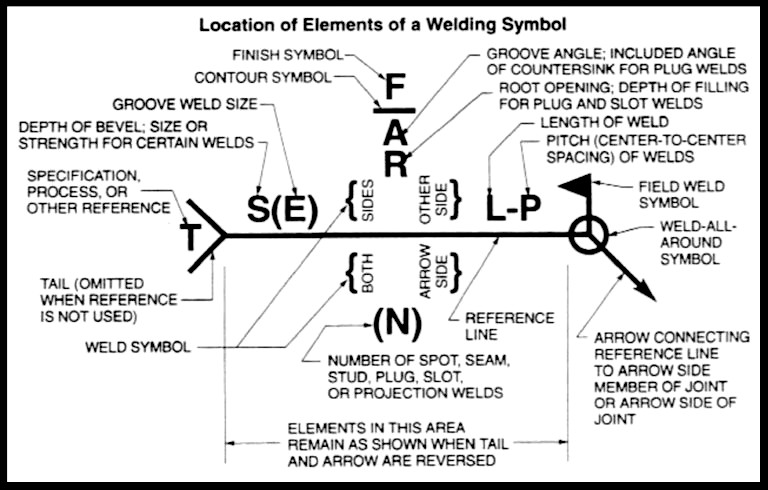
\includegraphics[scale=.7]{PIC/CH07/WS}
\end{figure}
Some additional notes shall be explained.
\begin{itemize}
\item The letters CP in the tail of the arrow indicate a complete penetration butt weld.
\item The tail should be omitted if no reference T is required.
\item The size of a fillet weld shall be to the left of the symbol. The vertical line on the fillet weld symbol is \textbf{always} on the left.
\item For an incomplete penetration butt weld, the design throat thickness hsall be to the left of the symbol. Where no design throat thickness is shown, a complete penetration butt weld is assumed required.
\item Arrow side and other side welds are made the same size unless otherwise dimensioned.
\item Symbols only apply between abrupt changes in direction of welding unless governed by the `weld all round' symbol or otherwise dimensioned.
\end{itemize}

Weld symbols are summarized in the following table.
\begin{figure}[H]
\centering
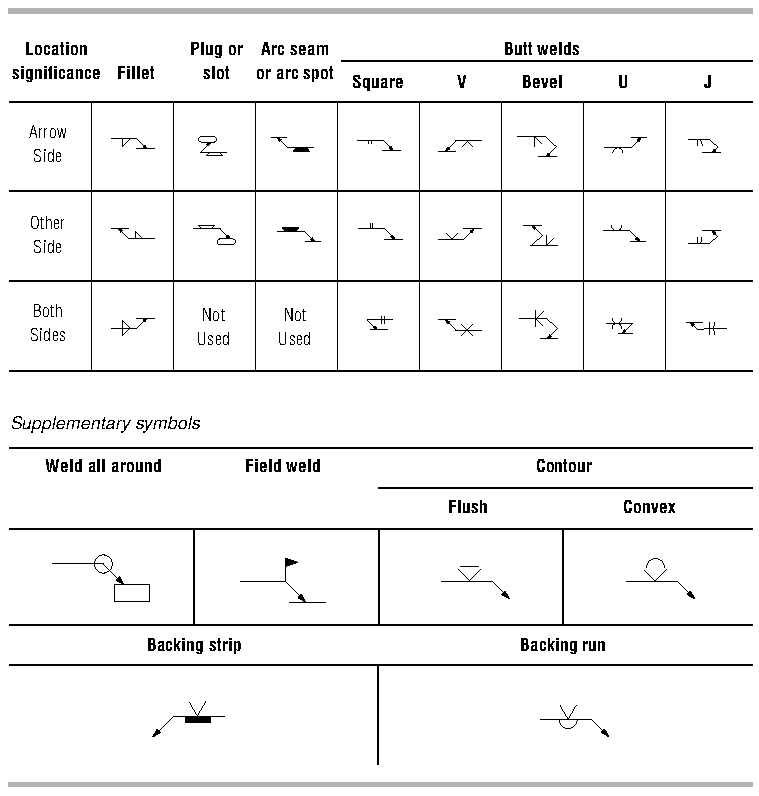
\includegraphics[width=.95\textwidth]{PIC/CH07/WST}
\caption{Welding symbols \citep{Gorenc2015}}
\end{figure}
\begin{figure}[p]
\centering
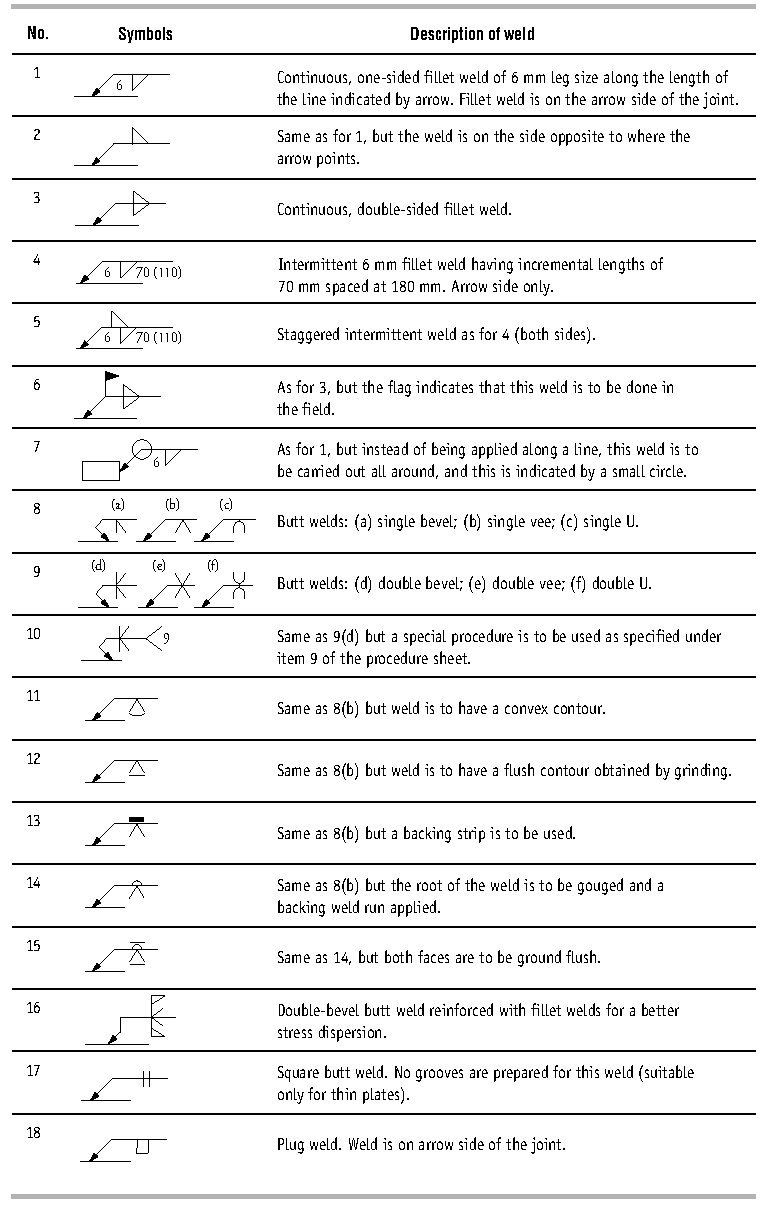
\includegraphics[width=.9\textwidth]{PIC/CH07/WUE}
\caption{Examples of use of welding symbols \citep{Gorenc2015}}
\end{figure}

The following are some examples of welding symbols taken from \citep{Corgan2017} on drawings and their physical meanings. All units are inches.
\begin{figure}[H]
\centering
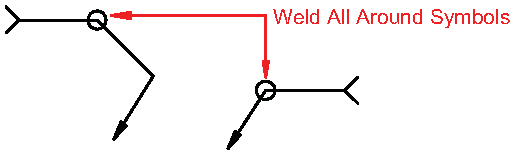
\includegraphics{PIC/CH07/EXAMPLE/WAR}
\caption{Weld all around welds \citep{Corgan2017}}
\end{figure}
\begin{figure}[H]
\centering
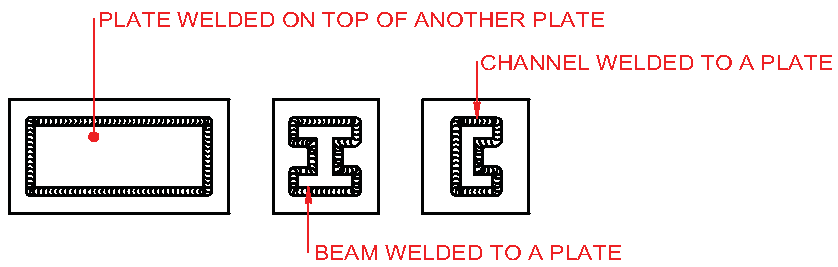
\includegraphics{PIC/CH07/EXAMPLE/WAR2}
\caption{Examples of weld all around welds \citep{Corgan2017}}
\end{figure}
\begin{figure}[H]
\centering
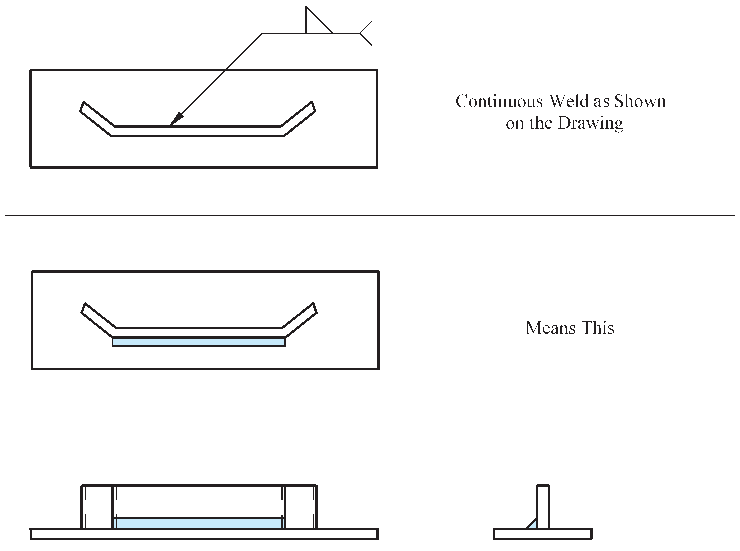
\includegraphics{PIC/CH07/EXAMPLE/CW}
\caption{Examples of continuous welds \citep{Corgan2017}}
\end{figure}
\begin{figure}[H]
\centering
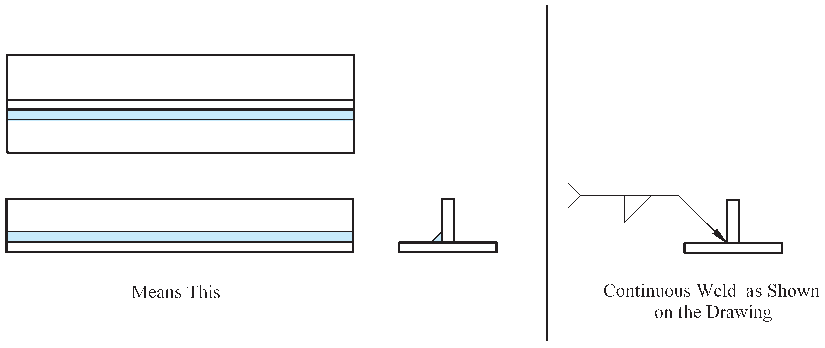
\includegraphics{PIC/CH07/EXAMPLE/CW1}
\caption{Examples of continuous welds \citep{Corgan2017}}
\end{figure}
\begin{figure}[H]
\centering
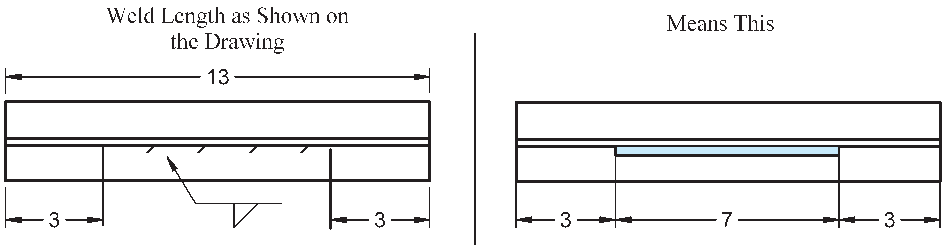
\includegraphics[width=.99\textwidth]{PIC/CH07/EXAMPLE/WL}
\caption{Weld length specified on welding symbol between extension lines (unit: inch) \citep{Corgan2017}}
\end{figure}
\begin{figure}[H]
\centering
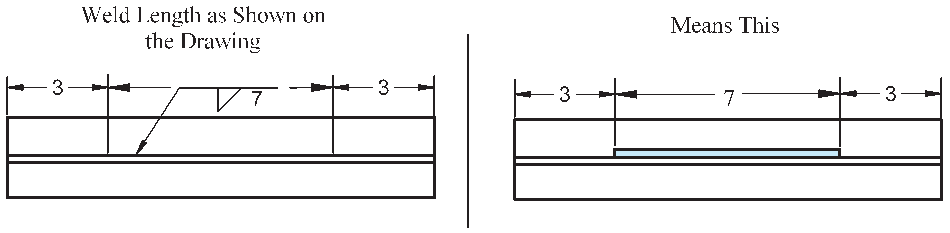
\includegraphics[width=.99\textwidth]{PIC/CH07/EXAMPLE/WL2}
\caption{Weld length specified on welding symbol between extension lines with
section lines representing the weld area (unit: inch) \citep{Corgan2017}}
\end{figure}
\begin{figure}[H]
\centering
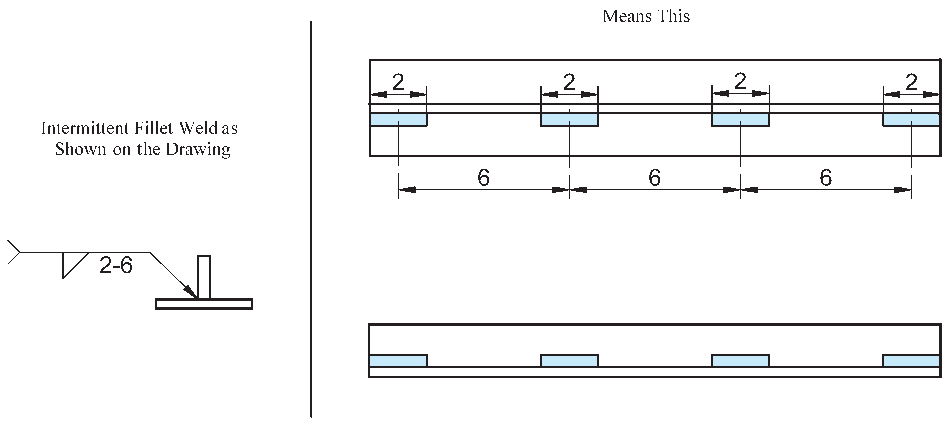
\includegraphics[width=.99\textwidth]{PIC/CH07/EXAMPLE/IW}
\caption{Example of intermittent welds (unit: inch) \citep{Corgan2017}}
\end{figure}
\begin{figure}[H]
\centering
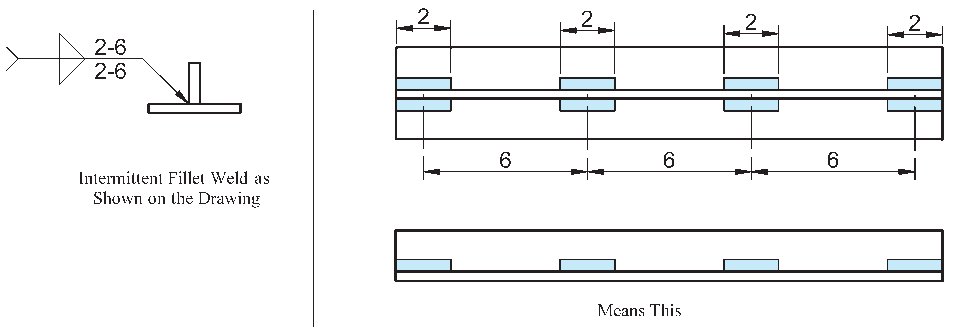
\includegraphics[width=.99\textwidth]{PIC/CH07/EXAMPLE/IW1}
\caption{Example of chain intermittent welds (unit: inch) \citep{Corgan2017}}
\end{figure}
\begin{figure}[H]
\centering
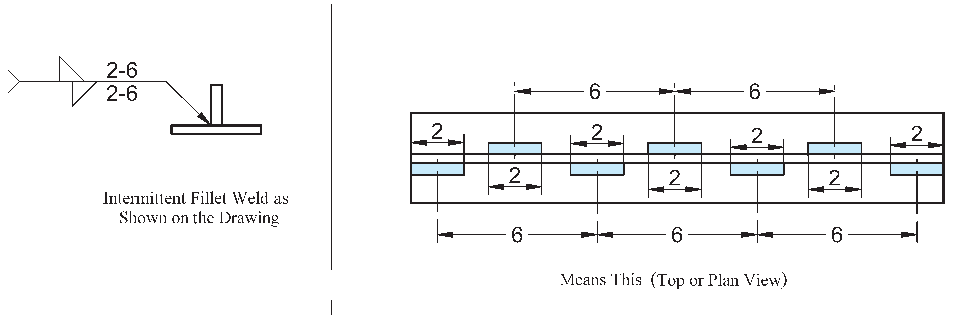
\includegraphics[width=.99\textwidth]{PIC/CH07/EXAMPLE/IW2}
\caption{Example of staggered intermittent welds (unit: inch) \citep{Corgan2017}}
\end{figure}
\begin{figure}[H]
\centering
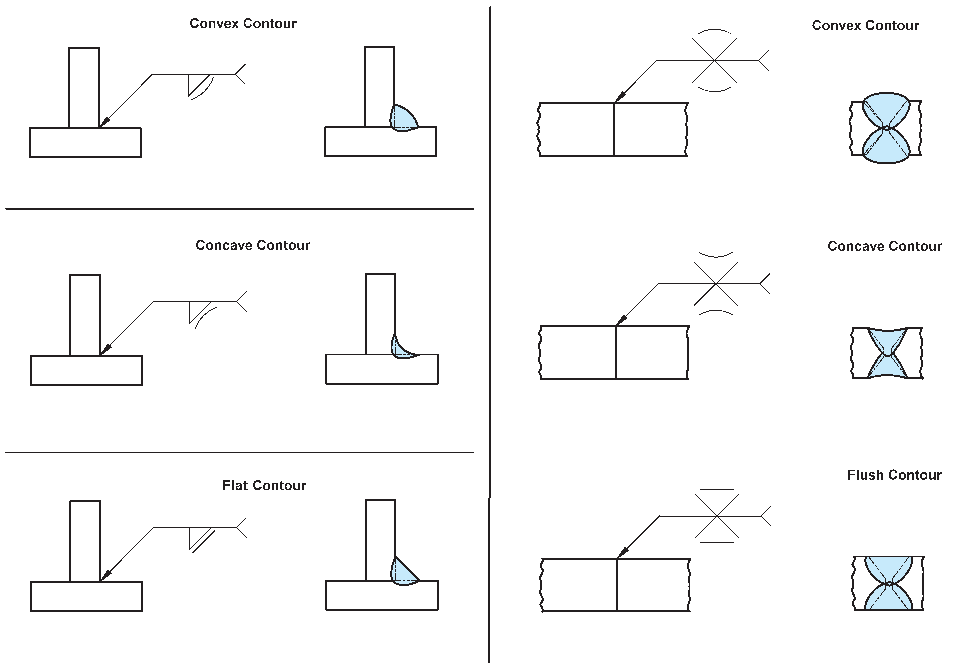
\includegraphics[width=.85\textwidth]{PIC/CH07/EXAMPLE/CS}
\caption{Contour symbols \citep{Corgan2017}}
\end{figure}
\begin{figure}[H]
\centering
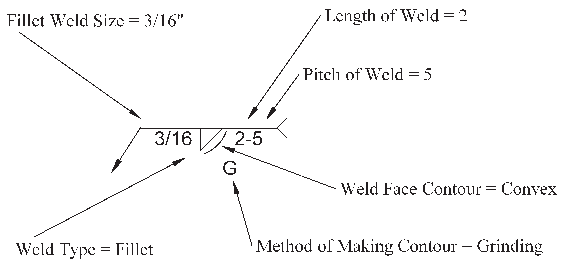
\includegraphics{PIC/CH07/EXAMPLE/FW}
\caption{Example of a welding symbol for a fillet weld (unit: inch) \citep{Corgan2017}}
\end{figure}
\begin{figure}[H]
\centering
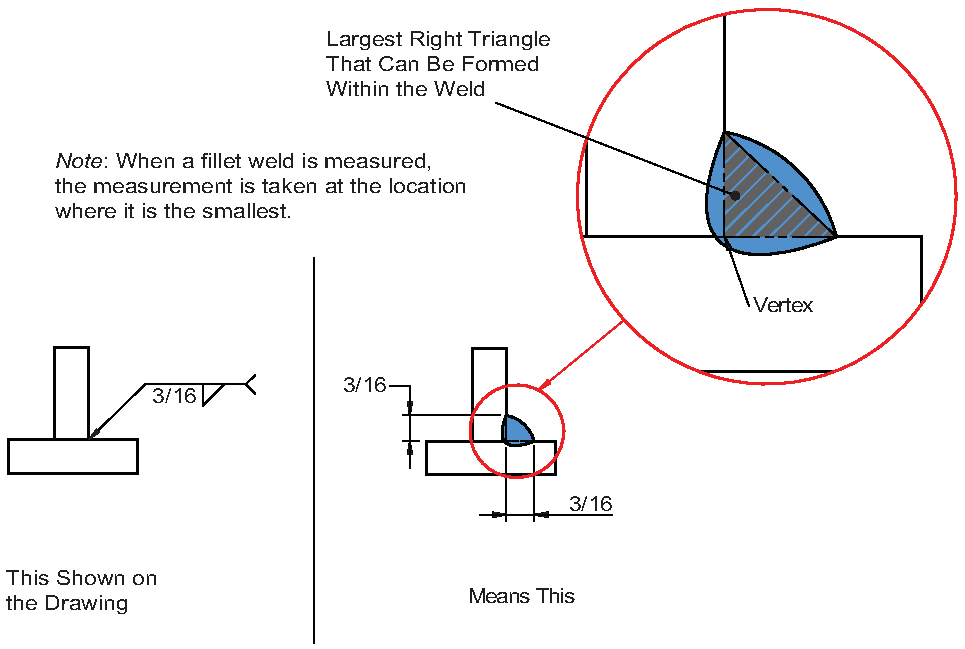
\includegraphics[width=.99\textwidth]{PIC/CH07/EXAMPLE/FWS}
\caption{Fillet weld size (unit: inch) \citep{Corgan2017}}
\end{figure}
\begin{figure}[H]
\centering
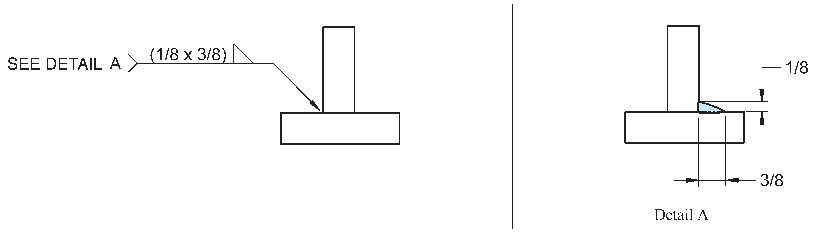
\includegraphics{PIC/CH07/EXAMPLE/UL}
\caption{Unequal leg fillet with detail drawing (unit: inch) \citep{Corgan2017}}
\end{figure}
\begin{figure}[H]
\centering
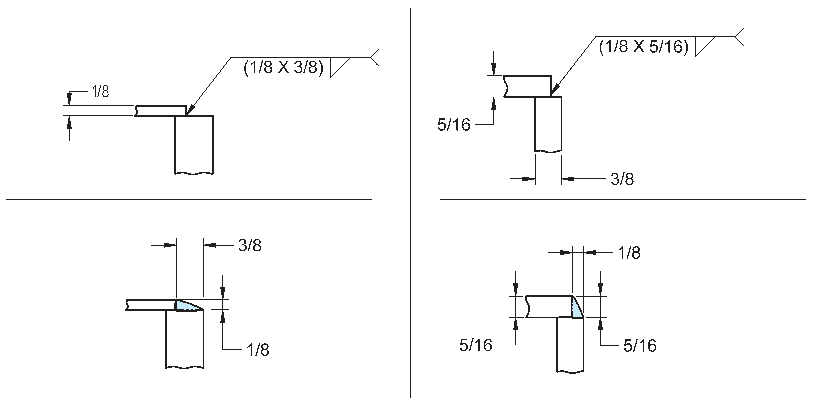
\includegraphics{PIC/CH07/EXAMPLE/UL2}
\caption{Unequal leg fillets that could be shown without detail (unit: inch) \citep{Corgan2017}}
\end{figure}
\begin{figure}[H]
\centering
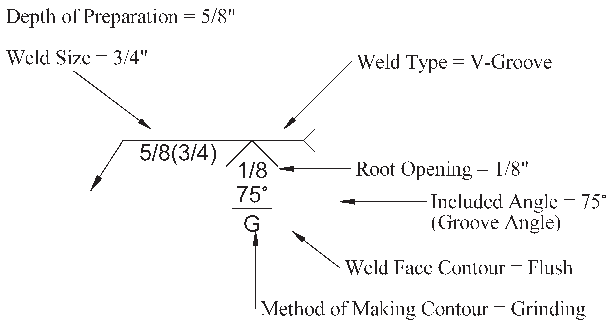
\includegraphics{PIC/CH07/EXAMPLE/BW}
\caption{Welding symbol example for a groove weld (unit: inch) \citep{Corgan2017}}
\end{figure}
\begin{figure}[H]
\centering
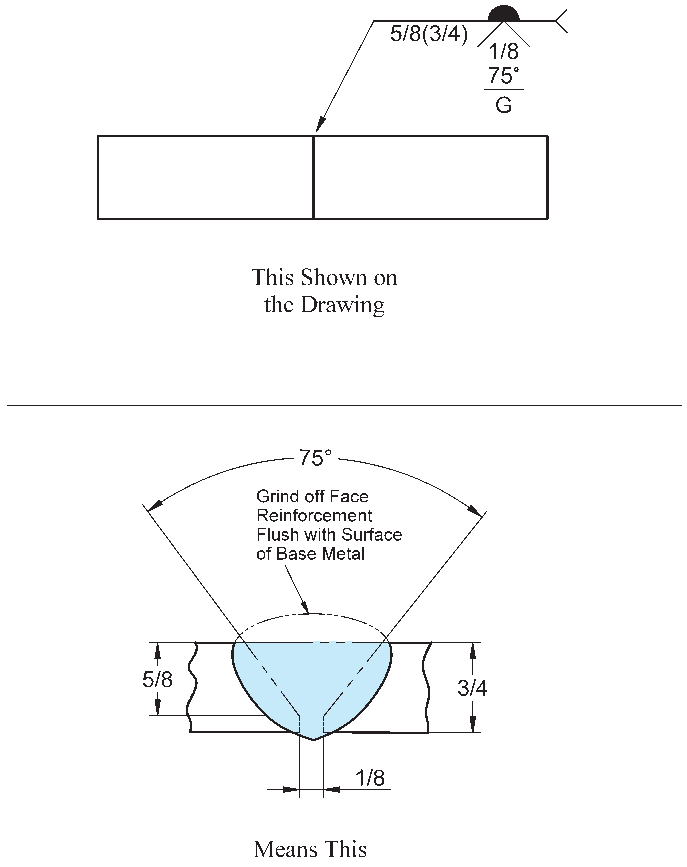
\includegraphics{PIC/CH07/EXAMPLE/BW2}
\caption{Example of a groove/butt weld (unit: inch) \citep{Corgan2017}}
\end{figure}
\begin{figure}[H]
\centering
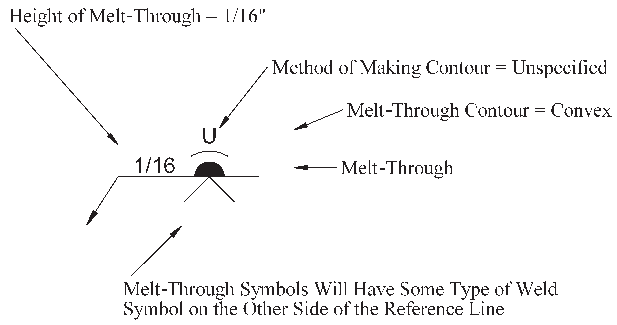
\includegraphics{PIC/CH07/EXAMPLE/MT}
\caption{Welding symbol with melt--through (unit: inch) \citep{Corgan2017}}
\end{figure}
\begin{figure}[H]
\centering
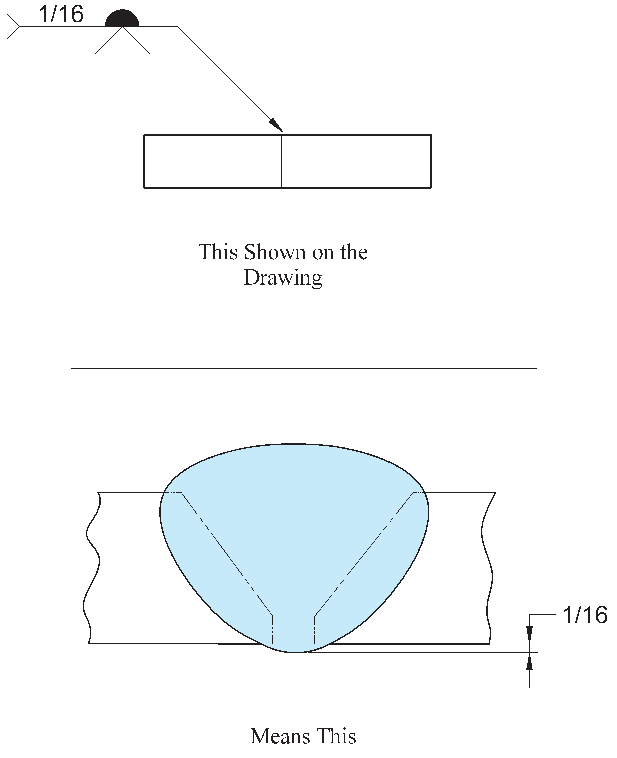
\includegraphics{PIC/CH07/EXAMPLE/MT2}
\caption{Melt--through example (unit: inch) \citep{Corgan2017}}
\end{figure}
\begin{figure}[p]
\centering
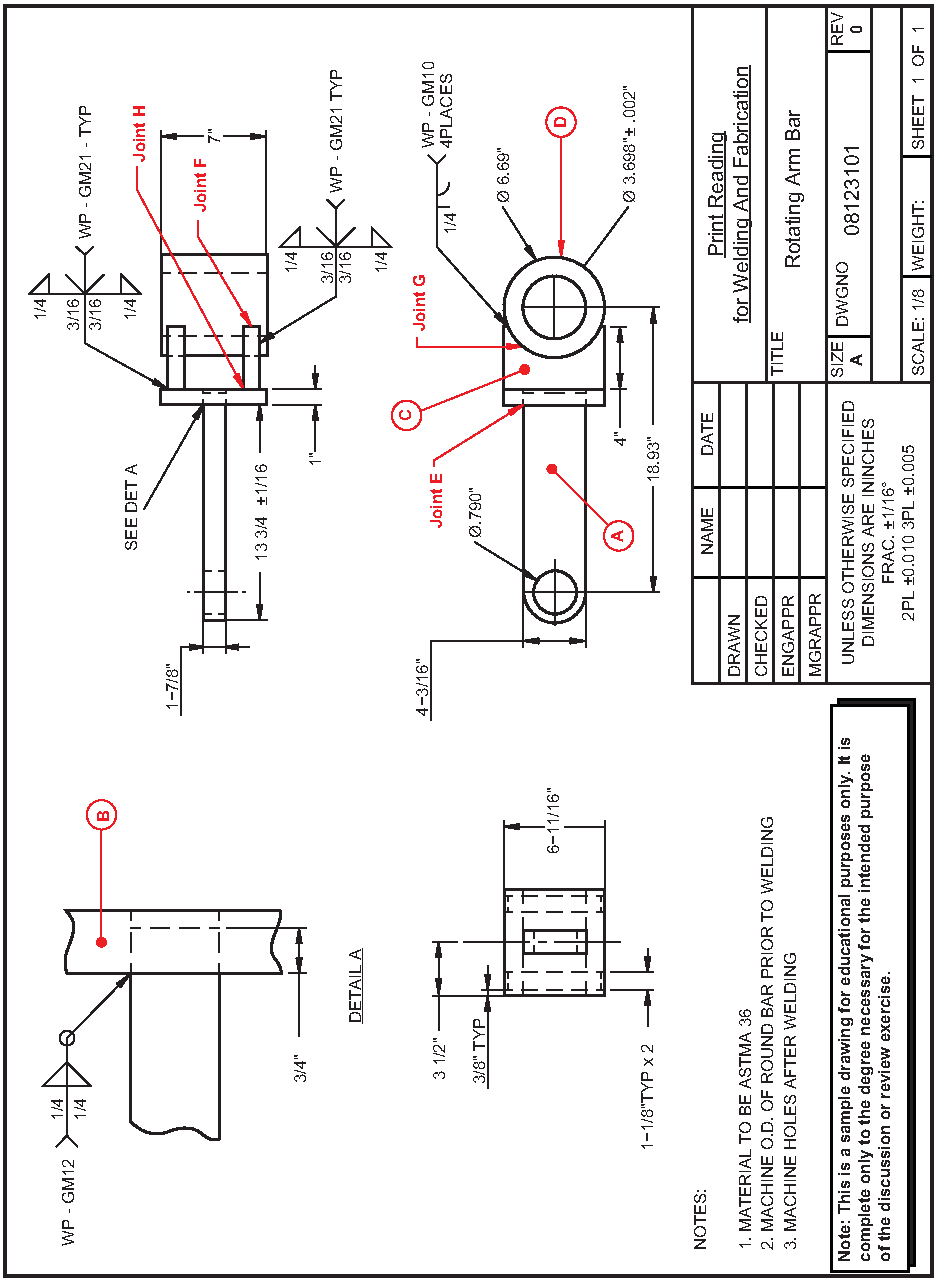
\includegraphics[width=.99\textwidth]{PIC/CH07/EXAMPLE/EX}
\end{figure}
\section{Electrodes Used for Welding}
\begin{table}[H]
\centering\footnotesize
\caption{Nominal tensile strength of weld metal ($f_{uw}$)}
\begin{tabular}{ccc}
	\toprule
	MMAW  & SAW, FCAW, GMAW &    $f_{uw}$    \\ \midrule
	E41XX &      W40X       & \SI{410}{\mpa} \\
	E48XX &      W50X       & \SI{480}{\mpa} \\ \bottomrule
\end{tabular}
\end{table}
The values of `X' represent the usage, or they are related to the Charpy impact test. All of these welds may be used with Grade 250 to Grade 350 steel. This system is used in this book.

A new system of weld specification is available according to \ASNZSWELD{}.
\begin{table}[H]
\centering\footnotesize
\caption{Nominal tensile strength of weld metal ($f_{uw}$)}
\begin{tabular}{ccc}
	\toprule
	                          &       Symbol        &           $f_{uw}$           \\ \midrule
	\multirow{5}{*}{System A} &        A-E35        &        \SI{440}{\mpa}        \\
	                          &        A-E38        &        \SI{470}{\mpa}        \\
	                          &        A-E42        &        \SI{500}{\mpa}        \\
	                          &        A-E46        &        \SI{530}{\mpa}        \\
	                          &        A-E50        &        \SI{560}{\mpa}        \\ \midrule
	\multirow{4}{*}{System B} &        B-E43        &        \SI{430}{\mpa}        \\
	                          & \color{cc0066}B-E49 & \color{cc0066}\SI{490}{\mpa} \\
	                          &        B-E55        &        \SI{550}{\mpa}        \\
	                          &        B-E57        &        \SI{570}{\mpa}        \\ \bottomrule
\end{tabular}
\end{table}
System A is used in Europe (based on yield stress), while System B is based on ultimate stress and is more common in Australasia.

The industry standard welding strength is $f_{uw}=\SI{490}{\mpa}$, so this should be
specified in practice (where possible).
\section{Weld Size and Strength}
\begin{itemize}
\item \textbf{Butt Weld}\\Complete penetration butt weld should be the same thickness as the material they are connecting. By using an electrode of sufficient strength ($f_{uw}\geqslant{}f_u$) and an SP weld, the effect of the weld can be ignored since the weld strength does not limit the member strength.
\item \textbf{Fillet Weld}
\begin{itemize}
\item \textbf{Preferred Sizes}\\Preferred sizes of a fillet weld with $t_w$ less than \SI{15}{\mm} are \SI{2}{\mm}, \SI{4}{\mm}, \SI{5}{\mm}, \SI{6}{\mm}, \SI{8}{\mm}, \SI{10}{\mm} and \SI{12}{\mm} (\NZSSTEEL{\S~9.7.3.2}).
\item \textbf{Minimum Length}\\The minimum length $l_w$ is $4t_w$ to ensure good fusion.
\item \textbf{Minimum Size}
\begin{table}[H]
\centering\footnotesize\caption{Minimum size of fillet weld $t_w$}
\begin{tabular}{cc}
	\toprule
	Thickness of thickest part joined $t$ (\si{\mm}) & $t_w$ (\si{\mm}) \\ \midrule
	                 $t\leqslant7$                   &     \num{3}      \\
	                $7<t\leqslant10$                 &     \num{4}      \\
	               $10<t\leqslant15$                 &     \num{5}      \\
	                     $15<t$                      &     \num{6}      \\ \bottomrule
\end{tabular}
\end{table}
\item \textbf{Maximum Size}
\begin{table}[H]
\centering\footnotesize\caption{Maximum size of fillet weld $t_w$}
\begin{tabular}{cc}
	\toprule
	Thickness of material alongside which fillet weld is to be made $t$ (\si{\mm}) & $t_w$ (\si{\mm}) \\ \midrule
	                                    $t<6$                                      &       $t$        \\
	                               $6\geqslant{}t$                                 &      $t-1$       \\ \bottomrule
\end{tabular}
\end{table}
This is necessary to a) prevent yielding of base material and b) indicate actual throat thickness.
\end{itemize}
\end{itemize}

The \textbf{weld strength per unit length} shall satisfy (\NZSSTEEL{\S~9.7.3.10})
\begin{gather}
v_w^*\leqslant\phi{}v_w=\phi{}0.6f_{uw}t_tk_r,
\end{gather}
where
\begin{conditions}
\phi&strength reduction factor\\
&\num{0.8} for SP\\
&\num{0.6} for GP\\
v_w^*&vectorial summation of design force per unit length on weld effective area\\
v_w&nominal capacity of a fillet weld per unit length\\
f_{uw}&nominal tensile strength of weld material\\
0.6f_{uw}&nominal shear strength of weld material\\
t_t&design throat thickness, usually equal to $t_w/\sqrt{2}$ where $t_w$ is the leg length, or fillet weld size\\
k_r&reduction factor for welded lap connection (otherwise $k_r=1.0$)\\
&\num{1.00} if $l_w\leqslant\SI{1.7}{\meter}$\\
&$1.10-0.06L_w$ if $\SI{1.7}{\meter}<l_w\leqslant\SI{8.0}{\meter}$\\
&\num{0.62} if $l_w>\SI{8.0}{\meter}$
\end{conditions}
\begin{figure}[H]
\centering\footnotesize
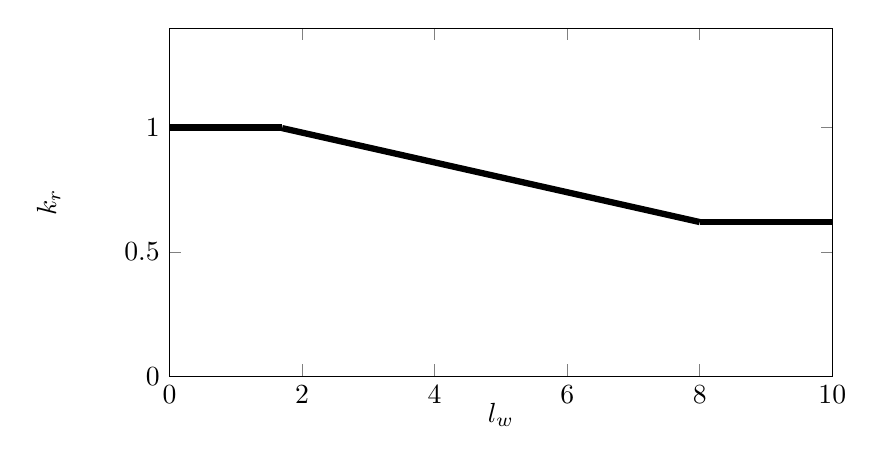
\begin{tikzpicture}
\begin{axis}[
width=10cm,height=6cm,
xlabel=$l_w$,
ylabel=$k_r$,
x label style={at={(axis description cs:0.5,-0.05)},anchor=north},
y label style={at={(axis description cs:-0.15,.5)},anchor=south},
xmin=0,
ymin=0,
xmax=10,
ymax=1.4,
]
\addplot[domain=0:1.7,samples=2,line width=.8mm]({x},1);
\addplot[domain=1.7:8,samples=2,line width=.8mm]({x},{1.1-.06*x});
\addplot[domain=8:10,samples=2,line width=.8mm]({x},.62);
\end{axis}
\end{tikzpicture}
\caption{$k_r$ as a function of $l_w$}
\end{figure}
\begin{figure}[H]
\centering
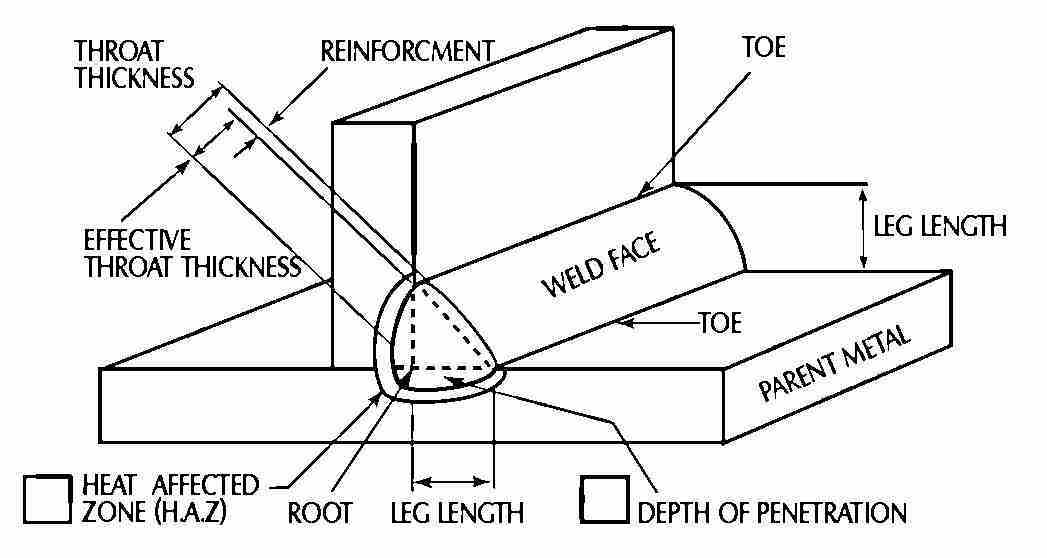
\includegraphics[width=8cm]{PIC/CH07/WTERM}
\caption{Weld terminology (\href{http://mdme.atspace.com/modules/7759G_Mechanical_Design/welds/Welded_Joints.html}{\url{http://mdme.atspace.com/modules/7759G_Mechanical_Design/welds/Welded_Joints.html}})}
\end{figure}

Fillet welds can be loaded with components of force in shear ($\tau_y\approx\sigma_y/\sqrt{3}$) and tension/compression ($\sigma_y$). Design conservatively considers that the strength is based on $\tau_y\approx0.6\sigma_y$ for all components of loading.

\begin{figure}[H]
\centering
\footnotesize
\begin{tikzpicture}
\node at(-4,2){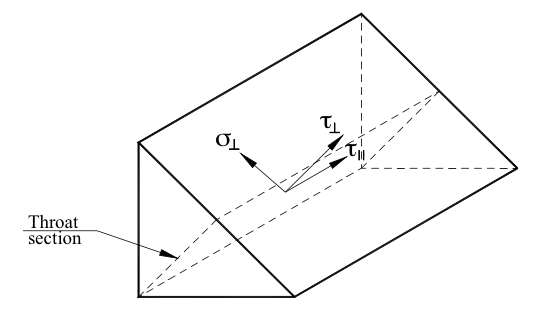
\includegraphics[width=6cm]{PIC/CH07/WSS}};
\draw(0,3)|-(3,0);
\draw[pattern=north east lines](2,0)--(0,2)|-cycle;
\draw(0,3)--++(20:5)coordinate(A)
(0,2)--++(20:5)coordinate(B)
(2,0)--++(20:5)coordinate(C)
(3,0)--++(20:5)coordinate(D);
\draw(A)--(B)--(C)--(D);
\dimline[extension start length=0,extension end length=0]{(0,-.5)}{(2,-.5)}{$t_w$};
\dimline[extension start length=0,extension end length=0]{(0,0)}{(1,1)}{$t_t$}
\dimline[extension start length=0,extension end length=0]{(3,0)}{($(3,0)+(20:5)$)}{$l_w$}
\end{tikzpicture}
\caption{Weld stress components (\href{https://offshorestructures.wordpress.com/2014/11/02/welded-lap-joints/}{\url{https://offshorestructures.wordpress.com/2014/11/02/welded-lap-joints/}})}
\end{figure}
The vectorial summation of design force per unit length can be associated with the stress components shown as follows. This is considered in some other standards with the strengths in each component direction (e.g., shear or tension).
\begin{gather}
v_w^*=t_t\sqrt{\sigma_\perp^2+\tau_\perp^2+\tau_\parallel^2}
\end{gather}
\begin{table}[H]
\centering\footnotesize
\caption{Dependable capacities of equal leg fillet welds $\phi{}v_w$ (\si{\kn\per\mm}) with $k_r=1.0$}\label{tab:phi_v_w}
\begin{tabular}{c|c|c|c|c|c|c}
    \toprule
      $t_w$    &  \multicolumn{3}{c|}{GP Welds}  &  \multicolumn{3}{c}{SP Welds}   \\
    (\si{\mm}) & E41XX/W40X & E48XX/W50X & E49XX & E41XX/W40X & E48XX/W50X & E49XX \\ \midrule
        3      &   0.313    &   0.367    & 0.374 &   0.417    &   0.489    & 0.499 \\
        4      &   0.417    &   0.489    & 0.499 &   0.557    &   0.652    & 0.665 \\
        5      &   0.522    &   0.611    & 0.624 &   0.696    &   0.815    & 0.832 \\
        6      &   0.626    &   0.733    & 0.748 &   0.835    &   0.978    & 0.998 \\
        8      &   0.835    &   0.978    & 0.998 &   1.113    &   1.303    & 1.330 \\
        10     &   1.044    &   1.222    & 1.247 &   1.392    &   1.629    & 1.663 \\
        12     &   1.252    &   1.466    & 1.497 &   1.670    &   1.955    & 1.996 \\ \bottomrule
\end{tabular}
\end{table}

For example, for $t_w=\SI{3}{\mm}$, SP with E41XX electrodes, the dependable strength per unit length of weld is
\begin{align*}
\phi{}v_w&=0.8\times0.6\times\SI{410}{\mpa}\times\dfrac{\SI{3}{\mm}}{\sqrt{2}}\times1.0\\
&=\SI{0.417}{\kn\per\mm}.
\end{align*}

When using SP longitudinal fillet welds to RHS with $t<\SI{3}{\mm}$, SP capacities should be multiplied by \num{0.7}/\num{0.8} to account for the different $\phi$ factors.

Welds greater than \SI{8}{\mm} require multiple passes and tend to be less economical.
\section{Fillet Weld Root Gaps}
Where there is a separation/gap between plates (i.e., root gaps), the fillet weld size, $t_w$, is given by the inscribed triangle (which does not include the root gap) as shown (\NZSSTEEL{\S~9.7.3.1} and AS/NZS 5131 \S~7.5.8).
\begin{figure}[H]
\centering\footnotesize
\begin{tikzpicture}
\draw[fill=black!10](0,3)rectangle(-1.2,0);
\draw[thick](0,2.2)to[out=-47,in=135](1,1)to[out=-45,in=137](2.4,-.2)-|cycle;
\draw[pattern=north east lines](2,0)--(0,2)|-cycle;
\dimline[extension start length=0,extension end length=0]{(-1.5,0)}{(-1.5,2)}{$t_w$};
\dimline[extension start length=0,extension end length=0]{(-1.5,0)}{(-1.5,-.2)}{};
\draw[fill=black!10](-1.8,-.2)rectangle(3.5,-1.4);
\draw[<-](-1.9,-.1)--++(-1,0)node[fill=white]{gap};
\draw[<-](.4,1.2)--++(2,1)node[fill=white]{inscribed triangle};
\dimline[extension start length=0,extension end length=0]{(0,0)}{(1,1)}{$t_t$};
\end{tikzpicture}
\caption{Fillet weld with root gap}
\end{figure}

Fabrication tolerances are given in AS/NZS 5131 \S~7.5.8 Appendix F and \NZSSTEEL{\S~14.4}. Design/construction documentation should be clear as to how root gaps are considered (e.g., by the designer accounting for the tolerances with an increased $t_w$, or by the fabricator).
\section{Good Practice for Welded Members}
Although not shown in \NZSSTEEL{}, the following are some good practice for welded members.
\begin{itemize}
\item It is good practice to use end returns. The effective length $L_e$ includes returns.
\begin{figure}[H]
\centering\footnotesize
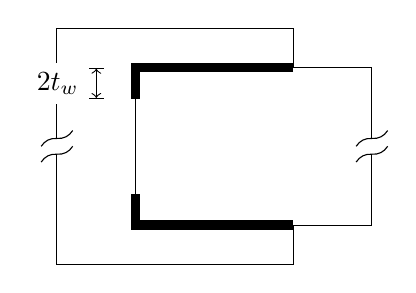
\begin{tikzpicture}[scale=1,ext/.pic={
\path[fill=white](-0.2,0)to[bend left](0,0.1)to[bend right](0.2,0.2)to(0.2,0)to[bend left](0,-0.1)to[bend right](-0.2,-0.2)--cycle;
\draw(-0.2,0)to[bend left](0,0.1)to[bend right](0.2,0.2) (0.2,0)to[bend left](0,-0.1)to[bend right](-0.2,-0.2);
}]
\draw(2,-1.5)rectangle(-1,1.5);
\draw[fill=white](0,-1)rectangle(3,1);
\draw(3,0)pic{ext};
\draw(-1,0)pic{ext};
\draw[line width=1.2mm](2,1)-|(0,.6)(2,-1)-|(0,-.6);
\draw[|<->|](-.5,.6)--(-.5,1)node[midway,left=1mm,fill=white]{$\geqslant2t_w$};
\end{tikzpicture}
\end{figure}
\item For flat bars with only longitudinal fillet welds, make $L>W$, to minimise stress concentration.
\begin{figure}[H]
\centering\footnotesize
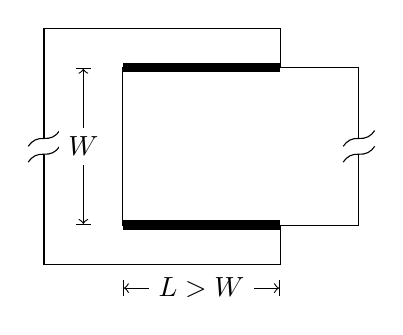
\begin{tikzpicture}[scale=1,ext/.pic={
\path[fill=white](-0.2,0)to[bend left](0,0.1)to[bend right](0.2,0.2)to(0.2,0)to[bend left](0,-0.1)to[bend right](-0.2,-0.2)--cycle;
\draw(-0.2,0)to[bend left](0,0.1)to[bend right](0.2,0.2) (0.2,0)to[bend left](0,-0.1)to[bend right](-0.2,-0.2);
}]
\draw(2,-1.5)rectangle(-1,1.5);
\draw[fill=white](0,-1)rectangle(3,1);
\draw(3,0)pic{ext};
\draw(-1,0)pic{ext};
\draw[line width=1.2mm](2,1)--(0,1)(2,-1)--(0,-1);
\draw[|<->|](2,-1.8)--++(-2,0)node[midway,fill=white]{$L>W$};
\draw[|<->|](-.5,-1)--++(0,2)node[midway,fill=white]{$W$};
\end{tikzpicture}
\end{figure}
\item For weld placement in connections subject to repeated stress, center of weld resistance should coincide with member centroid unless special allowance is made for the eccentricity.
\begin{figure}[H]
\centering\footnotesize
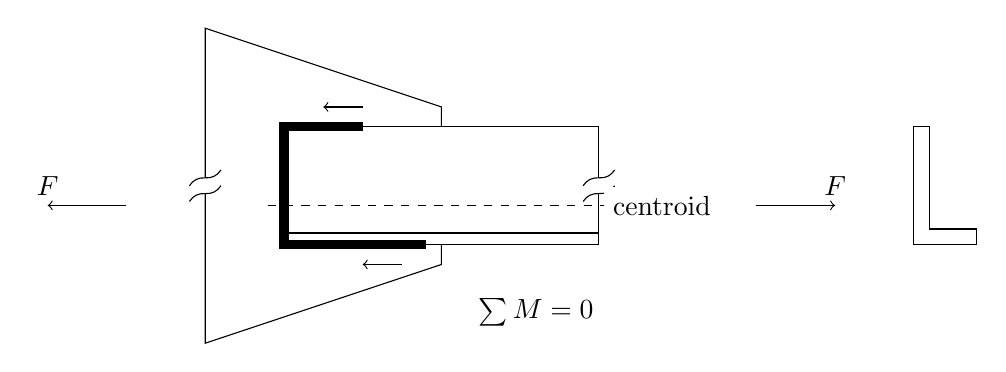
\begin{tikzpicture}[scale=1,ext/.pic={
\path[fill=white](-0.2,0)to[bend left](0,0.1)to[bend right](0.2,0.2)to(0.2,0)to[bend left](0,-0.1)to[bend right](-0.2,-0.2)--cycle;
\draw(-0.2,0)to[bend left](0,0.1)to[bend right](0.2,0.2) (0.2,0)to[bend left](0,-0.1)to[bend right](-0.2,-0.2);
}]
\draw(2,-1)--(2,1)--(-1,2)--(-1,-2)--cycle;
\draw[fill=white](0,-.75)rectangle(4,.75);
\draw(0,-.6)--(4,-.6);
\draw(4,0)pic{ext};
\draw(-1,0)pic{ext};
\draw[dashed](-.2,-.25)--++(5,0)node[fill=white]{centroid};
\draw[line width=1.2mm](1,.75)-|(0,-.75)--++(1.8,0)node[below right=5mm]{$\sum{}M=0$};
\draw[->](-2,-.25)--++(-1,0)node[above]{$F$};
\draw[->](6,-.25)--++(1,0)node[above]{$F$};
\draw[->](1,1)--++(-.5,0);
\draw[->](1.5,-1)--++(-.5,0);
\begin{scope}[xshift=8cm]
\draw(0,-.75)|-(.2,.75)|-(.8,-.55)|-cycle;
\end{scope}
\end{tikzpicture}
\end{figure}
\item For plug and slotted holes, make ends rounded to avoid stress concentration.
\begin{figure}[H]
\centering\footnotesize
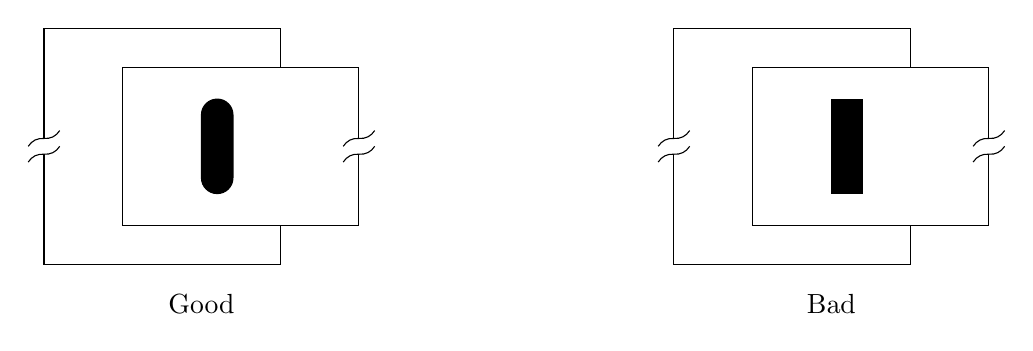
\begin{tikzpicture}[scale=1,ext/.pic={
\path[fill=white](-0.2,0)to[bend left](0,0.1)to[bend right](0.2,0.2)to(0.2,0)to[bend left](0,-0.1)to[bend right](-0.2,-0.2)--cycle;
\draw(-0.2,0)to[bend left](0,0.1)to[bend right](0.2,0.2) (0.2,0)to[bend left](0,-0.1)to[bend right](-0.2,-0.2);
}]
\draw(2,-1.5)rectangle(-1,1.5);
\draw[fill=white](0,-1)rectangle(3,1);
\draw(3,0)pic{ext};
\draw(-1,0)pic{ext};
\draw[rounded corners=2mm,fill=black](1,-.6)rectangle++(.4,1.2);
\node at(1,-2){Good};
\begin{scope}[xshift=8cm]
\draw(2,-1.5)rectangle(-1,1.5);
\draw[fill=white](0,-1)rectangle(3,1);
\draw(3,0)pic{ext};
\draw(-1,0)pic{ext};
\draw[fill=black](1,-.6)rectangle++(.4,1.2);
\node at(1,-2){Bad};
\end{scope}
\end{tikzpicture}
\end{figure}
\end{itemize}
\section{Member Design Considerations}
\subsection{Yielding on Gross Area}
This has been previously studied, see \eqsref{eq:tension_gross}.
\begin{gather}
N^*\leqslant\phi{}A_gf_y.
\end{gather}
\subsection{Fracture on Effective Net Area}
This has been previously studied, see \eqsref{eq:tension_net}.
\begin{gather}
N^*\leqslant\phi0.85k_{te}A_nf_u.
\end{gather}
\subsection{Block Tearing Failure}
Connections connected by welds should be checked for block tearing failure as for the bolted connections, see \S~\ref{sec:block_failure}.
\begin{figure}[H]
\centering\footnotesize
\begin{tikzpicture}[scale=1,ext/.pic={
\path[fill=white](-0.2,0)to[bend left](0,0.1)to[bend right](0.2,0.2)to(0.2,0)to[bend left](0,-0.1)to[bend right](-0.2,-0.2)--cycle;
\draw(-0.2,0)to[bend left](0,0.1)to[bend right](0.2,0.2) (0.2,0)to[bend left](0,-0.1)to[bend right](-0.2,-0.2);
}]
\draw(-1,-1.5)rectangle++(3,3);
\draw[dashed,fill=white](0,-1)rectangle++(3,2);
\draw(3,0)pic{ext};
\draw(-1,0)pic{ext};
\draw[line width=1.2mm](2,1)-|(0,-1)--++(2,0);
\draw[very thick,cc0066](.8,-1)rectangle++(3,2);
\draw[very thick,cc0066](3.8,0)pic{ext};
\draw[->,line width=.6mm](4.5,0)--++(1,0)node[right=2mm]{$N^*$};
\draw[->,line width=.6mm](-1.5,0)--++(-1,0)node[left=2mm]{$N^*$};
\end{tikzpicture}\caption{Block tear out of welded connection}
\end{figure}

Since there is no need to distinguish between gross and net areas for welded connections, assuming the plate has a uniform thickness $t_p$, it is possible to denote $A_v=A_{gv}=A_{nv}=l_vt_p$ and $A_t=A_{gt}=A_{nt}=l_tt_p$,  then \eqsref{eq:block_shear} becomes
\begin{align}
N^*\leqslant\phi0.95\left(0.6l_{v}+l_{t}\right)t_pf_u
\end{align}
\begin{conditions}
\phi&strength reduction factor, \num{0.9}\\
l_v&weld length subject to shear\\
l_t&weld length subject to tension\\
t_p&plate thickness
\end{conditions}

%\ANSI{J5.2} recommends the following guidelines. When a bolt that carries load passes through fillers that are equal to or less than \SI{6}{\mm} thick, the shear strength shall be used without reduction. When a bolt that carries load passes through fillers that are greater than \SI{6}{\mm} thick, one of the following requirements shall apply:
%\begin{enumerate}
%\item The shear strength of the bolts shall be multiplied by the factor
%\begin{gather}
%1-0.0154\left(t-6\right)
%\end{gather}
%but not less than \num{0.85}, where $t$ is the total thickness of the fillers.
%\item The fillers shall be welded or extended beyond the joint and bolted to uniformly distribute the total force in the connected element over the combined cross section of the connected element and the fillers.
%\item The size of the joint shall be increased to accommodate a number of bolts that is
%equivalent to the total number required in the previous requirement.
%\end{enumerate}
%
%Since this seldom governs, we will use the simplified method.
%\begin{gather}
%N^*\leqslant\phi0.85l_wt_p0.6f_u,
%\end{gather}
%where
%\begin{conditions}
%\phi&strength reduction factor, \num{0.9}\\
%l_w&weld length\\
%t_p&plate thickness
%\end{conditions}
\begin{exmp}
Fillet Weld Analysis

Find the strength of the connection shown if Grade 300 steel and E41XX electrodes are used for GP welds.
\begin{figure}[H]
\footnotesize
\begin{tikzpicture}[scale=1.4,x=1cm,y=1cm,ext/.pic={
\path[fill=exmpbg](-0.2,0)to[bend left](0,0.1)to[bend right](0.2,0.2)to(0.2,0)to[bend left](0,-0.1)to[bend right](-0.2,-0.2)--cycle;
\draw(-0.2,0)to[bend left](0,0.1)to[bend right](0.2,0.2) (0.2,0)to[bend left](0,-0.1)to[bend right](-0.2,-0.2);
}]
\draw(1.5,-1.5)rectangle(-1,1.5);
\draw[fill=exmpbg](0,-1)rectangle(3,1);
\draw(3,0)pic{ext};
\draw(-1,0)pic{ext};
\setstructmech{convention=direction}
\NodalForce{5,0}[N^*][N][N]
\NodalForce{-1.5,0}[-N^*][N][N]
\draw[line width=1.2mm](1.5,-1)-|(0,1)--++(1.5,0);
\draw[|<->|](0,-2)--(1.5,-2)node[midway,fill=exmpbg]{\SI{150}{\mm}};
\draw[|<->|](-.5,-1)--++(0,2)node[midway,fill=exmpbg,rotate=90]{\SI{200}{\mm}};
\draw[<-](1,-1.1)--(2,-1.4);
\draw[<-](1,.9)--(2,-1.4);
\draw[<-](.1,0)--(2,-1.4);
\draw(2,-1.4)--++(1,0)--++(-.3,-.3)--++(0,.3)node[below left=1mm and 2mm]{\num{10}};
\draw[<-](2.5,.5)--++(1,.5)--++(1,0)node[fill=exmpbg]{PL12\texttimes200};
\draw[<-](.5,1.3)--++(1,.5)--++(1,0)node[fill=exmpbg]{PL20\texttimes300};
\end{tikzpicture}
\end{figure}
\end{exmp}
\begin{solution}
\begin{enumerate}
\item
The effective throat thickness is
\begin{gather*}
t_t=\dfrac{\sqrt{2}}{2}\times{}t_w=\SI{7.07}{\mm}.
\end{gather*}
Weld capacity per unit length
\begin{align*}
\phi{}V_w&=\phi{}0.6f_{uw}t_tk_r\\
&=0.6\times0.6\times\SI{410}{\mpa}\times\SI{7.07}{\mm}\times1\\
&=\SI{1.044}{\kn\per\mm}.
\end{align*}
This value can be seen in \tabref{tab:phi_v_w}. The total capacity is then
\begin{gather*}
\SI{1.044}{\kn\per\mm}\times\SI{500}{\mm}=\SI{521.8}{\kn}.
\end{gather*}
\item
Check yielding of plate,
\begin{gather*}
\phi{}A_gf_y=0.9\times\SI{12}{\mm}\times\SI{200}{\mm}\times\SI{310}{\mpa}=\SI{669.6}{\kn}.
\end{gather*}
\item
Check fracture of plate,
\begin{gather*}
\phi0.85k_{te}A_nf_u=0.9\times0.85\times1\times\SI{12}{\mm}\times\SI{200}{\mm}\times\SI{430}{\mpa}=\SI{789.5}{\kn}.
\end{gather*}
\item
Check block tearing, note block tearing can only happen for PL20\texttimes300 plate,
\begin{align*}
&\phi0.95\left(0.6l_{v}+l_{t}\right)t_pf_u\\=&0.9\times0.95\times\left(0.6\times\SI{300}{\mm}+\SI{200}{\mm}\right)\times\SI{20}{\mm}\times\SI{430}{\mpa}\\
=&\SI{2794}{\kn}.
\end{align*}
\end{enumerate}
Thus weld strength governs, $N^*\leqslant\SI{521.8}{\kn}$.
\end{solution}

\begin{exmp} Determine the size and length of fillet weld for the lap joint of two Grade 300 steel plates with $N^*=\SI{640}{\kn}$ as shown. Assume plate yield and fracture requirements are satisfied, check block tearing.
\begin{figure}[H]
\footnotesize
\begin{tikzpicture}[scale=1,x=1cm,y=1cm,ext/.pic={
\path[fill=exmpbg](-0.2,0)to[bend left](0,0.1)to[bend right](0.2,0.2)to(0.2,0)to[bend left](0,-0.1)to[bend right](-0.2,-0.2)--cycle;
\draw(-0.2,0)to[bend left](0,0.1)to[bend right](0.2,0.2) (0.2,0)to[bend left](0,-0.1)to[bend right](-0.2,-0.2);
}]
\draw(2,-1.5)rectangle(-1,1.5);
\draw[fill=exmpbg](0,-1)rectangle(3,1);
\draw(3,0)pic{ext};
\draw(-1,0)pic{ext};
\setstructmech{convention=direction}
\NodalForce{5,0}[N^*][N][N]
\NodalForce{-1.5,0}[-N^*][N][N]
\draw[<-](2.5,.5)--++(1,.5)--++(1,0)node[fill=exmpbg]{PL16\texttimes175};
\draw[<-](.5,1.3)--++(1,.5)--++(2,0)node[fill=exmpbg]{\SI{16}{\mm} plate};
\end{tikzpicture}
\end{figure}
\end{exmp}
\begin{solution}
The maximum size of fillet weld is $t_w=t-\SI{1}{\mm}=\SI{15}{\mm}$.

The minimum size of fillet weld is $t_w=\SI{6}{\mm}$.

Try $\SI{6}{\mm}$ W40X SP weld, $L_{min}=4\times{}t_w=\SI{24}{\mm}$. Assume $k_r=1.0$, the capacity per unit length is
\begin{align*}
\phi{}v_w&=\phi{}0.6f_{uw}t_tk_r\\
&=0.8\times0.6\times\SI{410}{\mpa}\times\dfrac{\SI{6}{\mm}}{\sqrt{2}}\times1\\
&=\SI{0.835}{\kn\per\mm}.
\end{align*}
This value can be seen in \tabref{tab:phi_v_w}.

The weld length required is
\begin{gather*}
L_{min}=\dfrac{\SI{640}{\kn}}{\SI{0.835}{\kn\per\mm}}=\SI{766.5}{\mm}<\SI{1700}{\mm}.
\end{gather*}
Possible weld placements are the follows.
\begin{figure}[H]
\centering
\footnotesize
\begin{tikzpicture}[scale=1,ext/.pic={
\path[fill=exmpbg](-0.2,0)to[bend left](0,0.1)to[bend right](0.2,0.2)to(0.2,0)to[bend left](0,-0.1)to[bend right](-0.2,-0.2)--cycle;
\draw(-0.2,0)to[bend left](0,0.1)to[bend right](0.2,0.2) (0.2,0)to[bend left](0,-0.1)to[bend right](-0.2,-0.2);
}]
\draw(2,-1.5)rectangle(-1,1.5);
\draw[fill=exmpbg](0,-1)rectangle(3,1);
\draw(3,0)pic{ext};
\draw(-1,0)pic{ext};
\draw[line width=1.2mm](1.5,1)-|(0,-1)--++(1.5,0);
\begin{scope}[xshift=8cm]
\draw(2,-1.5)rectangle(-1,1.5);
\draw[fill=exmpbg](0,-1)rectangle(3,1);
\draw(3,0)pic{ext};
\draw(-1,0)pic{ext};
\draw[line width=1.2mm](2,1)-|(0,.8)(2,-1)-|(0,-.8);
\end{scope}
\end{tikzpicture}
\end{figure}
Which one is better?

Check block tearing using the first placement,
\begin{align*}
&\phi0.95\left(0.6l_{v}+l_{t}\right)t_pf_u\\=&0.9\times0.95\times\left(0.6\times\SI{591.5}{\mm}+\SI{175}{\mm}\right)\times\SI{16}{\mm}\times\SI{430}{\mpa}
\\=&\SI{3111}{\kn}>N^*=\SI{640}{\kn}.
\end{align*}

Check block tearing using the second placement,
\begin{align*}
&\phi0.95\left(0.6l_{v}+l_{t}\right)t_pf_u\\=&0.9\times0.95\times0.6\times\SI{766.5}{\mm}\times\SI{16}{\mm}\times\SI{430}{\mpa}
\\=&\SI{2705}{\kn}>N^*=\SI{640}{\kn}.
\end{align*}
\end{solution}
\begin{exmp}
Design fillet welds to develop the full strength of the angle below considering that it is subject to repeated loading. Use FCAW and Grade 350 steel.

Note that if no load is specified, then design connection to resist angle capacity.
\begin{figure}[H]
\footnotesize
\begin{tikzpicture}[scale=1,ext/.pic={
\path[fill=exmpbg](-0.2,0)to[bend left](0,0.1)to[bend right](0.2,0.2)to(0.2,0)to[bend left](0,-0.1)to[bend right](-0.2,-0.2)--cycle;
\draw(-0.2,0)to[bend left](0,0.1)to[bend right](0.2,0.2) (0.2,0)to[bend left](0,-0.1)to[bend right](-0.2,-0.2);
}]
\draw(2,-1)--(2,1)--(-1,2)--(-1,-2)--cycle;
\draw[<-](0,1)--++(1,.5)--++(2,0)node[fill=exmpbg]{\SI{10}{\mm} plate};
\draw[fill=exmpbg](0,-.75)rectangle(4,.75);
\draw[<-](2.5,.5)--++(1,.5)--++(2,0)node[fill=exmpbg]{150\texttimes100\texttimes10UA};
\draw(0,-.6)--(4,-.6);
\draw(4,0)pic{ext};
\draw(-1,0)pic{ext};
\draw[|<->|](5,-.75)--++(0,1.5)node[midway,fill=exmpbg]{\SI{150}{\mm}};
\draw[|<->|](6,-.75)--++(0,.5)node[midway,fill=exmpbg,right=2mm]{$y=\SI{48.1}{\mm}$};
\draw[dashed](-.2,-.25)--++(7,0)node[above=1mm]{N.A.};
\end{tikzpicture}
\end{figure}
\end{exmp}
\begin{solution}
\begin{enumerate}
\item Angle Capacity
\begin{gather*}
\phi{}A_gf_y=0.9\times\SI{2300}{\mm^2}\times\SI{360}{\mpa}=\SI{745}{\kn},\\
\phi0.85k_{te}A_nf_u=0.9\times0.85\times0.85\times\SI{2300}{\mm^2}\times\SI{480}{\mpa}=\SI{718}{\kn}.
\end{gather*}
Thus, $\phi{}N_t=\SI{718}{\kn}$.
\item Weld Length\\
The maximum size of fillet weld is $t_w=t-\SI{1}{\mm}=\SI{9}{\mm}$.

The minimum size of fillet weld is $t_w=\SI{4}{\mm}$.

Try $\SI{4}{\mm}$ W50X FCAW SP weld, $L_{min}=4\times{}t_w=\SI{16}{\mm}$. Assume $k_r=1.0$, the capacity per unit length is
\begin{align*}
\phi{}v_w&=\phi{}0.6f_{uw}t_tk_r\\
&=0.8\times0.6\times\SI{480}{\mpa}\times\dfrac{\SI{4}{\mm}}{\sqrt{2}}\times1\\
&=\SI{0.652}{\kn\per\mm}.
\end{align*}
The weld length required is
\begin{gather*}
L_{min}=\dfrac{\SI{718}{\kn}}{\SI{0.652}{\kn\per\mm}}=\SI{1101.6}{\mm}<\SI{1700}{\mm}.
\end{gather*}
\item Position of Welds\\
Balance welds so that there is no eccentricity.
\begin{figure}[H]
\centering
\footnotesize
\begin{tikzpicture}
\draw(0,-.75)rectangle(4,.75);
\draw(0,-.6)--(4,-.6);
\draw[|<->|](-1,-.75)--++(0,1.5)node[midway,fill=exmpbg]{\SI{150}{\mm}};
\draw[|<->|](5,-.75)--++(0,.5)node[midway,fill=exmpbg,right=2mm]{$y=\SI{48.1}{\mm}$};
\draw[dashed](-.2,-.25)--++(7,0)node[above=1mm]{N.A.};
\draw[line width=1.2mm](2,.75)-|(0,-.75)--++(3.5,0);
\draw[|<->|](0,1.25)--++(2,0)node[midway,fill=exmpbg,above=2mm]{$L_{w1}=\SI{278.2}{\mm}$};
\draw[|<->|](0,-1.25)--++(3.5,0)node[midway,fill=exmpbg]{$L_{w2}=\SI{673.4}{\mm}$};
\end{tikzpicture}
\end{figure}
Assume the top length is $L_{w1}$, take moment about N.A. of angle section,
\begin{align*}
\underbrace{L_{w1}\times\left(\SI{150}{\mm}-\SI{48.1}{\mm}\right)}_\text{top segment}&+\underbrace{\SI{150}{\mm}\times\left(\SI{150}{\mm}/2-\SI{48.1}{\mm}\right)}_\text{vertical segment}\\&=\underbrace{\left(\SI{1101.6}{\mm}-L_{w1}-\SI{150}{\mm}\right)\times\SI{48.1}{\mm}}_\text{bottom segment},
\end{align*}
this gives
\begin{gather*}
L_{w1}=\SI{278.2}{\mm},\qquad\text{use}\quad{}L_{w1}=\SI{280}{\mm},\\
L_{w2}=\SI{673.4}{\mm},\qquad\text{use}\quad{}L_{w2}=\SI{680}{\mm}.
\end{gather*}

Check block tearing, $l_v=L_{w1}+L_{w2}$,
\begin{align*}
&\phi0.95\left(0.6l_{v}+l_{t}\right)t_pf_u\\
=&0.9\times0.95\times\left(0.6\times\SI{960}{\mm}+\SI{150}{\mm}\right)\times\SI{10}{\mm}\times\SI{480}{\mpa}\\
=&\SI{2980}{\kn}>\phi{}N_t=\SI{717.9}{\kn}.
\end{align*}

All weld lengths are greater than $L_{min}$. Final layout.
\begin{figure}[H]
\centering
\footnotesize
\begin{tikzpicture}[ext/.pic={
\path[fill=exmpbg](-0.2,0)to[bend left](0,0.1)to[bend right](0.2,0.2)to(0.2,0)to[bend left](0,-0.1)to[bend right](-0.2,-0.2)--cycle;
\draw(-0.2,0)to[bend left](0,0.1)to[bend right](0.2,0.2) (0.2,0)to[bend left](0,-0.1)to[bend right](-0.2,-0.2);
}]
\draw(4,-1)--++(0,2)--(-1,2)--(-1,-2)--cycle;
\draw[fill=exmpbg](0,-.75)rectangle(8,.75);
\draw(0,-.6)--(8,-.6);
\draw[line width=1.2mm](2,.75)-|(0,-.75)--++(3.5,0);
\draw(1,.75)--++(1,1)--++(1.5,0)--++(-.3,-.3)node[left=1mm]{4}node[right=2mm]{280}--++(0,.3)--++(1.5,0)coordinate(A)node[right=2mm]{W50X SP};
\draw(A)--++(.2,.2);
\draw(A)--++(.2,-.2);
\draw(1.5,-.75)--++(1,-1)--++(1.5,0)--++(-.3,-.3)node[left=1mm]{4}node[right=2mm]{680}--++(0,.3)--++(.5,0);
\draw(0,0)--++(-1,-1)--++(-1,0)--++(0,-.3)node[left=1mm]{4}node[right=2mm]{150}--++(.3,.3)--++(-.5,0);
\draw(8,0)pic{ext}(-1,0)pic{ext};
\end{tikzpicture}
\end{figure}
\end{enumerate}
\end{solution}
\section{Quality of Welded Connection}
The quality of welded connections depends on
\begin{itemize}
\item weldability of steel\\This is a measure of the ability to produce a crack--free and sound structural joint.
\item proper preparation of the welded connections\\This involves cleanliness and alignment.
\item proper procedures
\begin{itemize}
\item good welding positions
\begin{figure}[H]
\centering
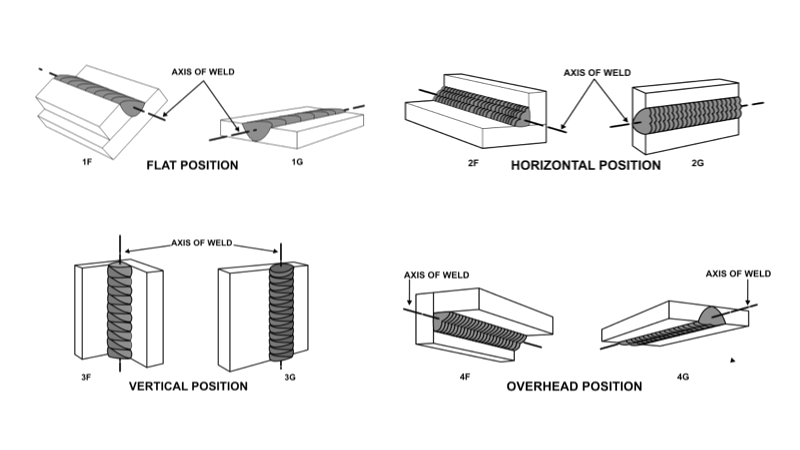
\includegraphics[width=14cm]{PIC/CH07/WP}
\caption{Weld positions (\href{https://weldguru.com/welding-positions/}{\url{https://weldguru.com/welding-positions/}})}
\end{figure}
\item control of distortion of the welded member
\begin{figure}[H]
\centering
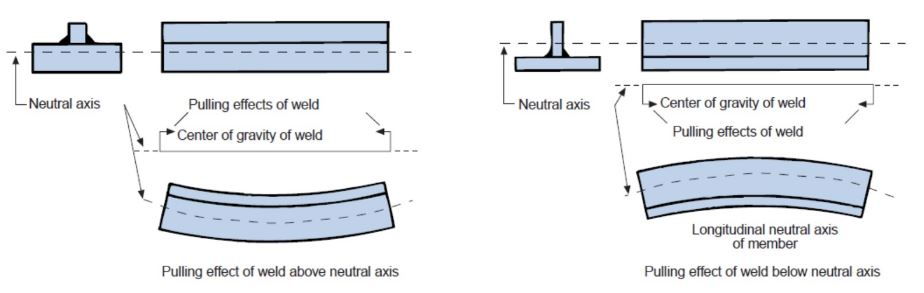
\includegraphics[width=14cm]{PIC/CH07/WD}
\caption{Weld distortion (\href{https://weldinganswers.com/7-ways-to-control-distortion-in-welding/}{\url{https://weldinganswers.com/7-ways-to-control-distortion-in-welding/}})}
\end{figure}
\begin{figure}[H]
\centering
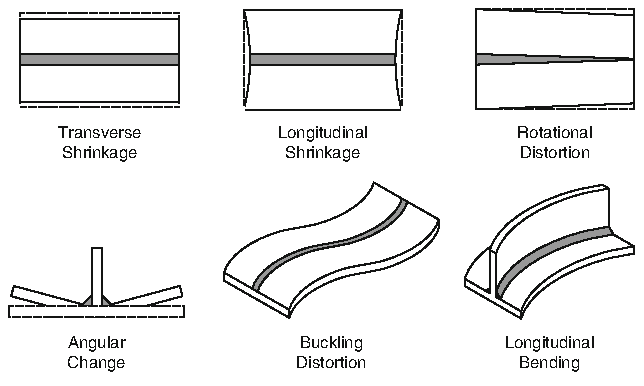
\includegraphics{PIC/CH07/WDD}
\caption{Weld distortion \citep{Hetnarski2014}}
\end{figure}
\item welding sequences to limit distortion
\begin{figure}[H]
\centering
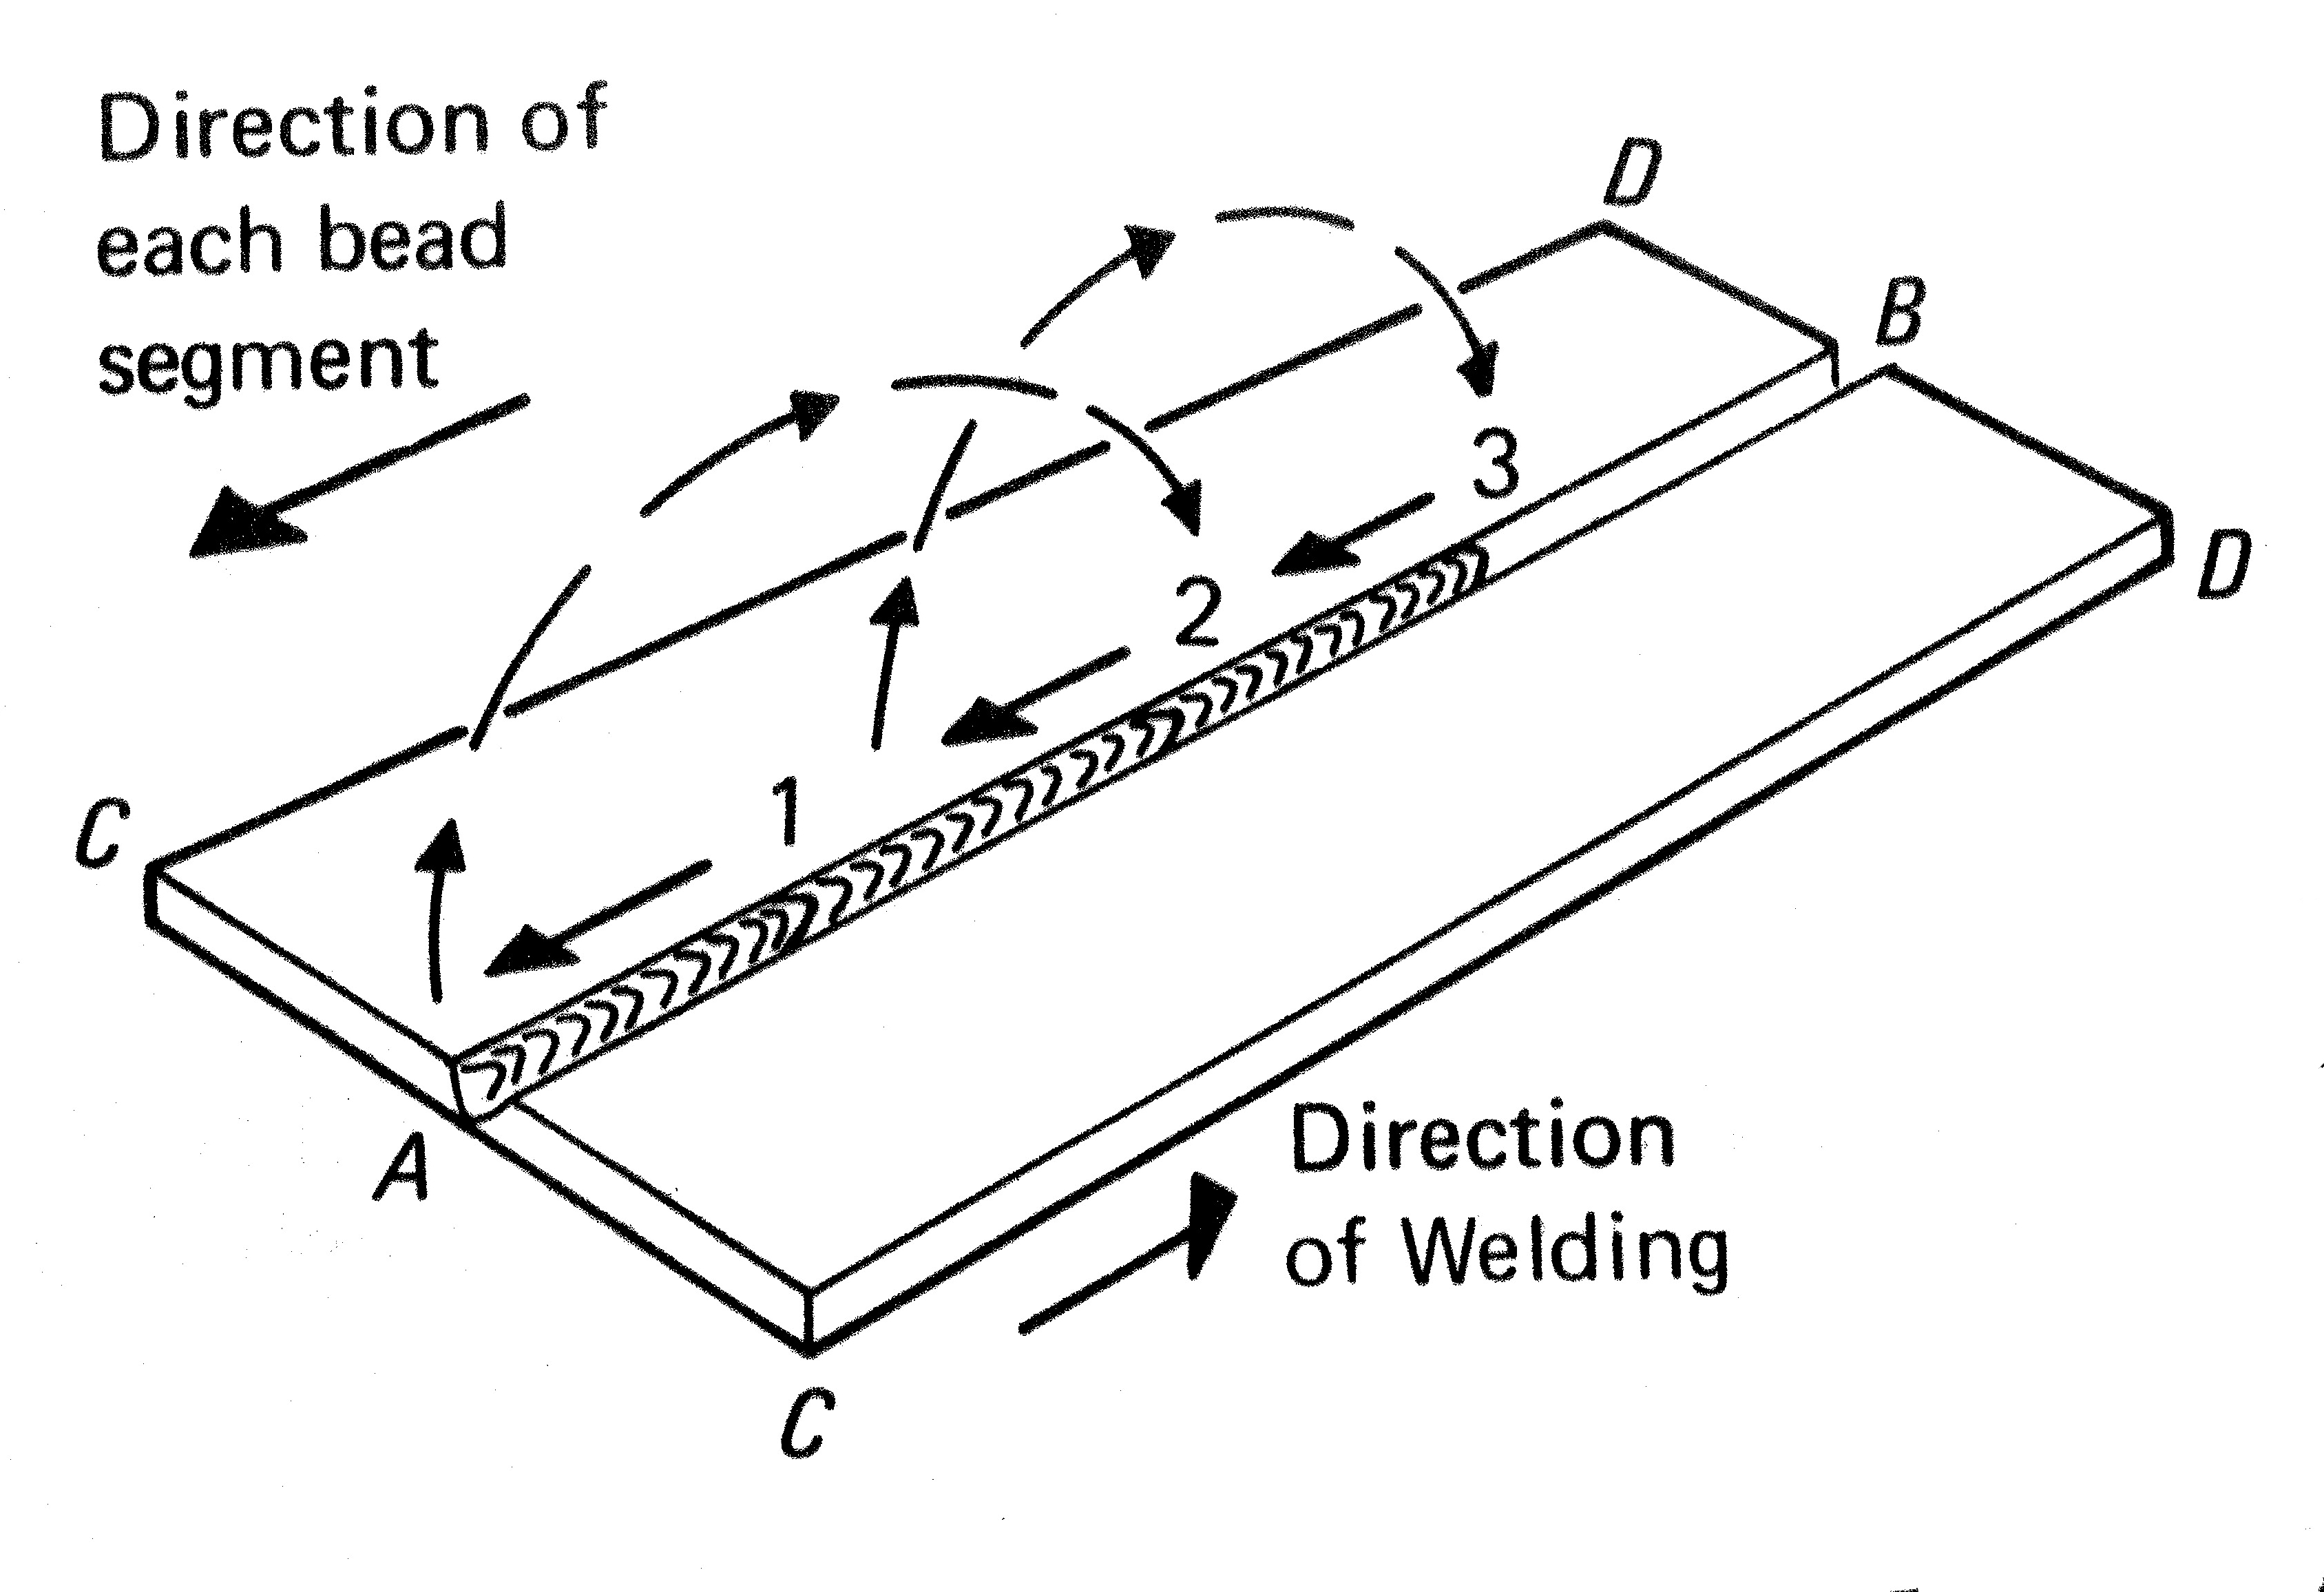
\includegraphics[width=12cm]{PIC/CH07/WSSS}
\caption{Back step weld (\href{https://www.fabricatingandmetalworking.com/2013/02/how-to-control-the-warping-of-parts-in-thin-sheet-metal/}{\url{https://www.fabricatingandmetalworking.com/2013/02/how-to-control-the-warping-of-parts-in-thin-sheet-metal/}})}
\end{figure}
\begin{figure}[H]
\centering
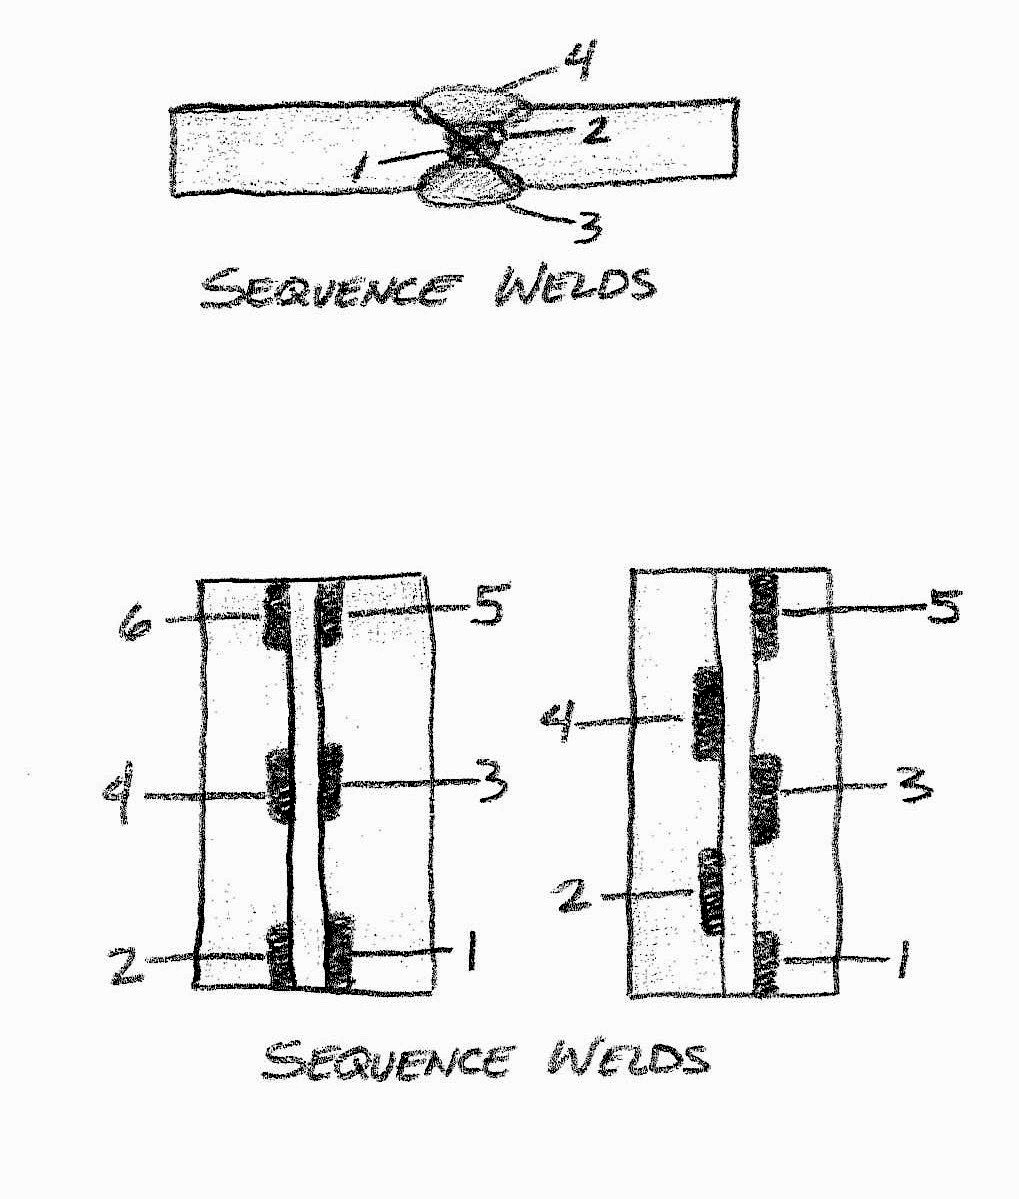
\includegraphics[height=12cm]{PIC/CH07/WSSSS}
\caption{Weld sequence (\href{https://axisfab.com/weld-shrinkage/}{\url{https://axisfab.com/weld-shrinkage/}})}
\end{figure}
\item minimum weld thickness
\item few passes
\begin{figure}[H]
\centering
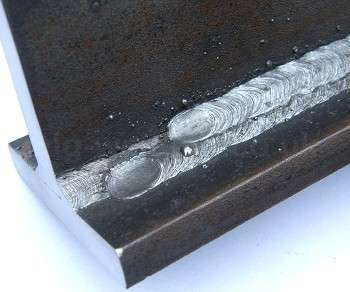
\includegraphics[scale=.8]{PIC/CH07/MPFW}
\caption{Multiple pass fillet weld (\href{https://www.mig-welding.co.uk/arc-fillet-joints.htm}{\url{https://www.mig-welding.co.uk/arc-fillet-joints.htm}})}
\end{figure}
\item correct current and voltage for weld material, correct rate of welding, etc.
\item correct electrode for type of steel chosen\\If weld material is much stronger than plate material then plate failure may occur. An electrode matching plate material is required.
\end{itemize}
\end{itemize}
\section{Possible Weld Defects}
Welds need to be inspected by ultrasound or other techniques to ensure that the performance of the connection will be adequate.

Interested readers can refer to this page\footnote{\url{https://www.theengineerspost.com/welding-defects/}} for full version.
\begin{itemize}
\item \textbf{Incomplete Fusion}\\These types of welding defects occur when there is a shortage of suitable fusion between the metal and weld. It may also be visible between adjacent weld beads. This produces a gap inside the joint that is not filled with molten metal.
\begin{figure}[H]
\centering
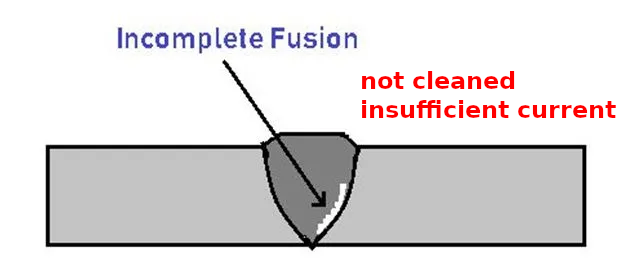
\includegraphics[scale=.3]{PIC/CH07/IF}
\end{figure}
\item \textbf{Incomplete Penetration}\\In these types of welding defects, penetration is defined as the distance from the uppermost surface of the base plate to the maximum extent of the weld nugget.

Incomplete penetration happens when the metal groove is not entirely filled, which means that the weld metal does not fully spread through the joint thickness.
\begin{figure}[H]
\centering
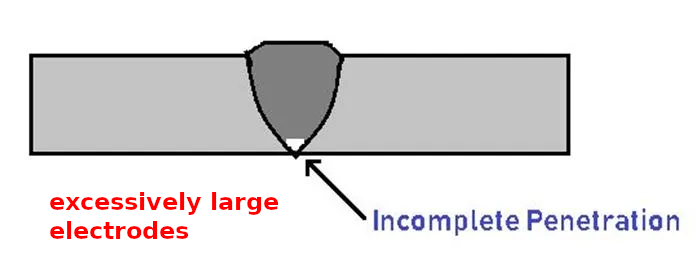
\includegraphics[scale=.3]{PIC/CH07/IP}
\end{figure}
\item \textbf{Porosity and Blowhole}\\Porosity is a group of small bubbles and blowholes are relatively large hidden holes or pores. They are mainly caused by trapped gases. Porosity is a result of weld metal contamination.
\begin{figure}[H]
\centering
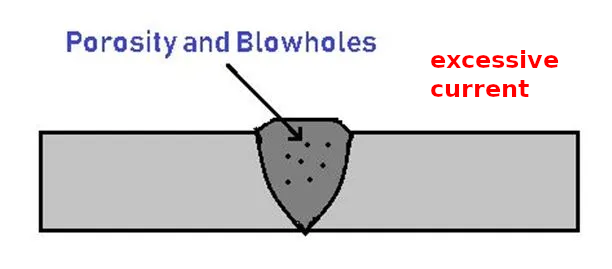
\includegraphics[scale=.3]{PIC/CH07/PB}
\end{figure}
\item \textbf{Undercut}\\Undercut in welding makes imperfection, it is the formation of grooves in the weld toe, which decreases the cross-sectional thickness of the base metal. As a result of this weld and workpiece get weakened.
\begin{figure}[H]
\centering
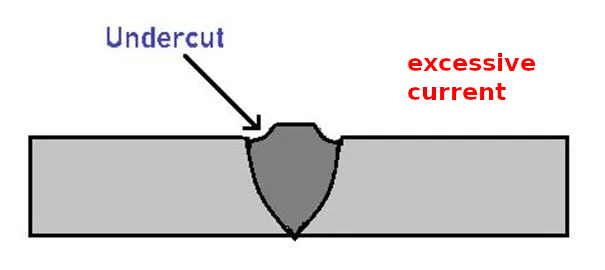
\includegraphics[scale=.3]{PIC/CH07/UC}
\end{figure}
\item \textbf{Slag Inclusion}\\Slag inclusion is welding defects that are usually visible in welds. The slag is a dangerous substance that appears as a product of stick welding, flux-core arc welding, and submerged arc welding.

It is can occur when the flux, which is a solid shielding material applied when welding, melts in the weld or on the surface of the weld region. Slag inclusion decreases the strength of the joint and hence makes it weaker.
\begin{figure}[H]
\centering
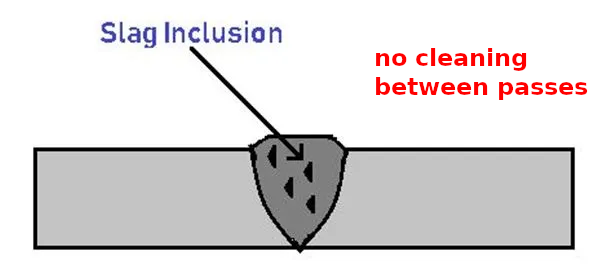
\includegraphics[scale=.3]{PIC/CH07/SI}
\end{figure}
\item \textbf{Weld Crack}\\These are the most dangerous types of welding defects. It is almost not allowed by all standards in the production. It can appear on the surface, in the weld metal, or in an area affected by strong heat.
\begin{figure}[H]
\centering
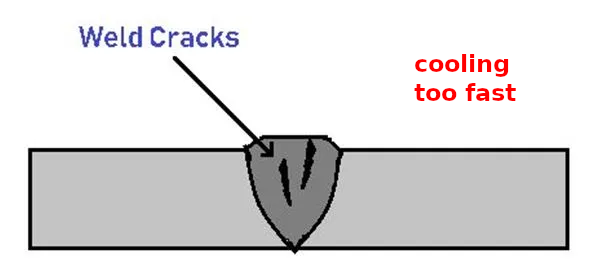
\includegraphics[scale=.3]{PIC/CH07/WC}
\end{figure}
\end{itemize}
\section{Possible Plate Defects}
\begin{figure}[H]
\centering
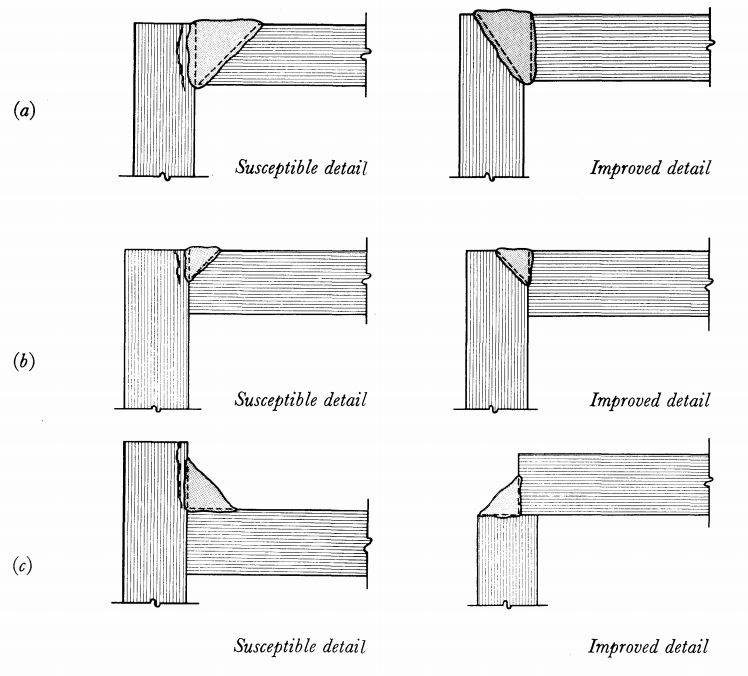
\includegraphics[width=.99\textwidth]{PIC/CH07/LT}
\caption{Susceptible and improved details (\href{https://buildingfailures.com/2014/11/28/overview-of-lamellar-tearing-and-representative-case-studies/}{\url{https://buildingfailures.com/2014/11/28/overview-of-lamellar-tearing-and-representative-case-studies/}})}
\end{figure}